%!TEX program=xelatex
%      "   
%    '':''
%   ___:____      |\/|
% ,'        `.    \  /
% |  O        \___/  |
% ~^~^~^~^~^~^~^~^~^~^

\documentclass[UTF8,a4paper,8pt,no-math]{article} %缺省为单栏
\usepackage[top=3cm,bottom=2cm,left=2cm,right=2cm]{geometry} % 页边距
\usepackage{ctex}
\usepackage{amsmath,amssymb,mathtools}
\usepackage{amsthm,mathrsfs}
\usepackage{graphicx} %引入宏包,就可以使用\includegrapics命令插图了.
\usepackage{supertabular}
\usepackage[dvipsnames]{xcolor}
\usepackage{float}
\usepackage{bbding} %特殊符号宏包
\usepackage{cases}
\usepackage{listings} %代码块

\usepackage{booktabs}
\usepackage{multirow}
\usepackage{colortbl}
\usepackage{diagbox}
\usepackage{enumerate}
\usepackage{arydshln}
\usepackage{xargs}
\usepackage{tcolorbox} % 彩色盒子
\tcbuselibrary{skins , breakable , listings ,theorems}

\usepackage[colorlinks,
	linkcolor=purple, % 目录,交叉引用颜色
	anchorcolor=blue,
	citecolor=blue]{hyperref}
\usepackage{url}
\title{杂谈勾股定理}
\author{tau}
%\date{\today}

\newtheorem{thm}{定理}[section]%定义一个thm环境,编号层次为section
\newtheorem{definition}{定义}[section]
\newtheorem{lemma}{引理}[thm]%编号紧接定理
\newtheorem{corollary}{推论}[thm]
\numberwithin{equation}{section} %公式编号,层次为section

% 自定义命令
\newcommand{\upcite}[1]{\textsuperscript{\cite{#1}}}  %自定义新命令\upcite, 使参考文献引用以上标出现
\newcommand{\ue}{\mathrm{e}} % 自定义命令\ue,数学环境直体自然底数e

\newcommand\norm[1]{\left\|#1\right\|} % 一个参数
\newcommand\dv[3][]{\frac{\mathrm{d}^{#1} #2}{\mathrm{d} #3^{#1}}} %一个默认参数
\newcommandx\seq[3][1=1,2=n,usedefault]{#3_{#1}\cdots #3_{#2}} %多个默认参数(需要xargs宏包)

\newcommand{\BB}{\mathbb{B}}
\newcommand{\thetab}{\boldsymbol{\theta}}

\graphicspath{{./image/}} %图片搜索路径,可以有多个,每一个用花括号括起

\bibliographystyle{plain}  %声明参考文献格式

% tcolorbox提供的theorme
\newtcbtheorem[number within=section]{mytheo}{定理}{colback=Emerald!10,colframe=cyan!40!black,fonttitle=\bfseries}{th}

\newtcbtheorem[number within=section]{mydef}{定义}{colback=JungleGreen!10!Cerulean!15,colframe=CornflowerBlue!60!Black,fonttitle=\bfseries}{th}

\newtcbtheorem[use counter from=mytheo]{mylemma}{引理}{colback=JungleGreen!10!Cerulean!15,colframe=CornflowerBlue!60!Black,fonttitle=\bfseries}{th}
% =======================================
% +			正文区						 +							
% +						      			+
% =======================================

\begin{document} %环境一般格式 \begin{环境名}[可选参数](其他参数)\end{环境名}

\maketitle            %命令输出论文题目
\tableofcontents      %命令输出目录

\begin{abstract}      %摘要环境
	这是一篇关于勾股定理的小文章.
\end{abstract}

{\color{NavyBlue}\section{勾股定理在古代}}   %开始新的一节 不同颜色字体需要宏包xcolor[dvipsnames].
称勾股定理为毕达哥拉斯定理,将勾股定理的发现归功于公元前6世纪的毕达哥拉斯学派.\cite{Kline}
该学派得到了一个法则,可以求出可排成直角三角形三边的三元数组.毕达哥拉斯学派没有书面著作,该定理的严格表述和证明见于欧几里得\footnote{欧几里得,约公元前330--275 年.}%脚注,花括号内是命令的参数,即脚注的内容
《几何原本》的命题47:“直角三角形斜边上的正方形等于两直角边上的两个正方形之和.”证明是用面积做的.

我国《周髀算经》载商高(约公元前12世纪)答周公问:
\begin{quote}      %quote环境(并不改变引用内容字体) 引用
	\zihao{-5}\kaishu  %改变字体,字号小5,楷书,以下接引用内容.(不能在内容之后)
	勾广三,股修四,径隅五.
\end{quote}
又载陈子(约公元前7--6世纪)答荣方问:
\begin{quote}
	\zihao{-5}\kaishu
	若求邪至日者,以日下为勾,日高为股,勾股各自乘,并而开方除之,得邪至日.
\end{quote}
都较古希腊更早.后者已经明确道出勾股定理的一般形式.
图 \ref{fig:xiantu} 是我国古代对勾股定理的一种证明\upcite{quanjing}.

\begin{figure}[ht]%figuer环境就是插图使用的浮动环境,有可选参数ht
	\centering     %表示后面的内容居中
	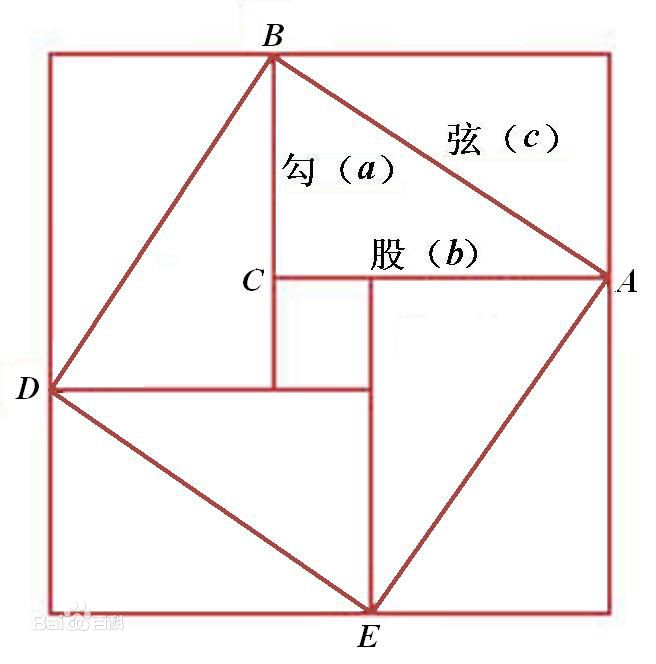
\includegraphics[scale=0.2]{xiantu.jpg} %插入图形,源文件所在目录图片名称.
	\caption{\kaishu 宋赵爽在《周髀算经》注中作的弦图(仿制),该图给出了勾股定理一个极具对称美的证明}%该命令给插图加上自动编号和标题.
	\label{fig:xiantu}  %交叉引用
\end{figure}

\begin{figure}[htbp]
	\begin{center}
		\begin{tabular}{cc}
			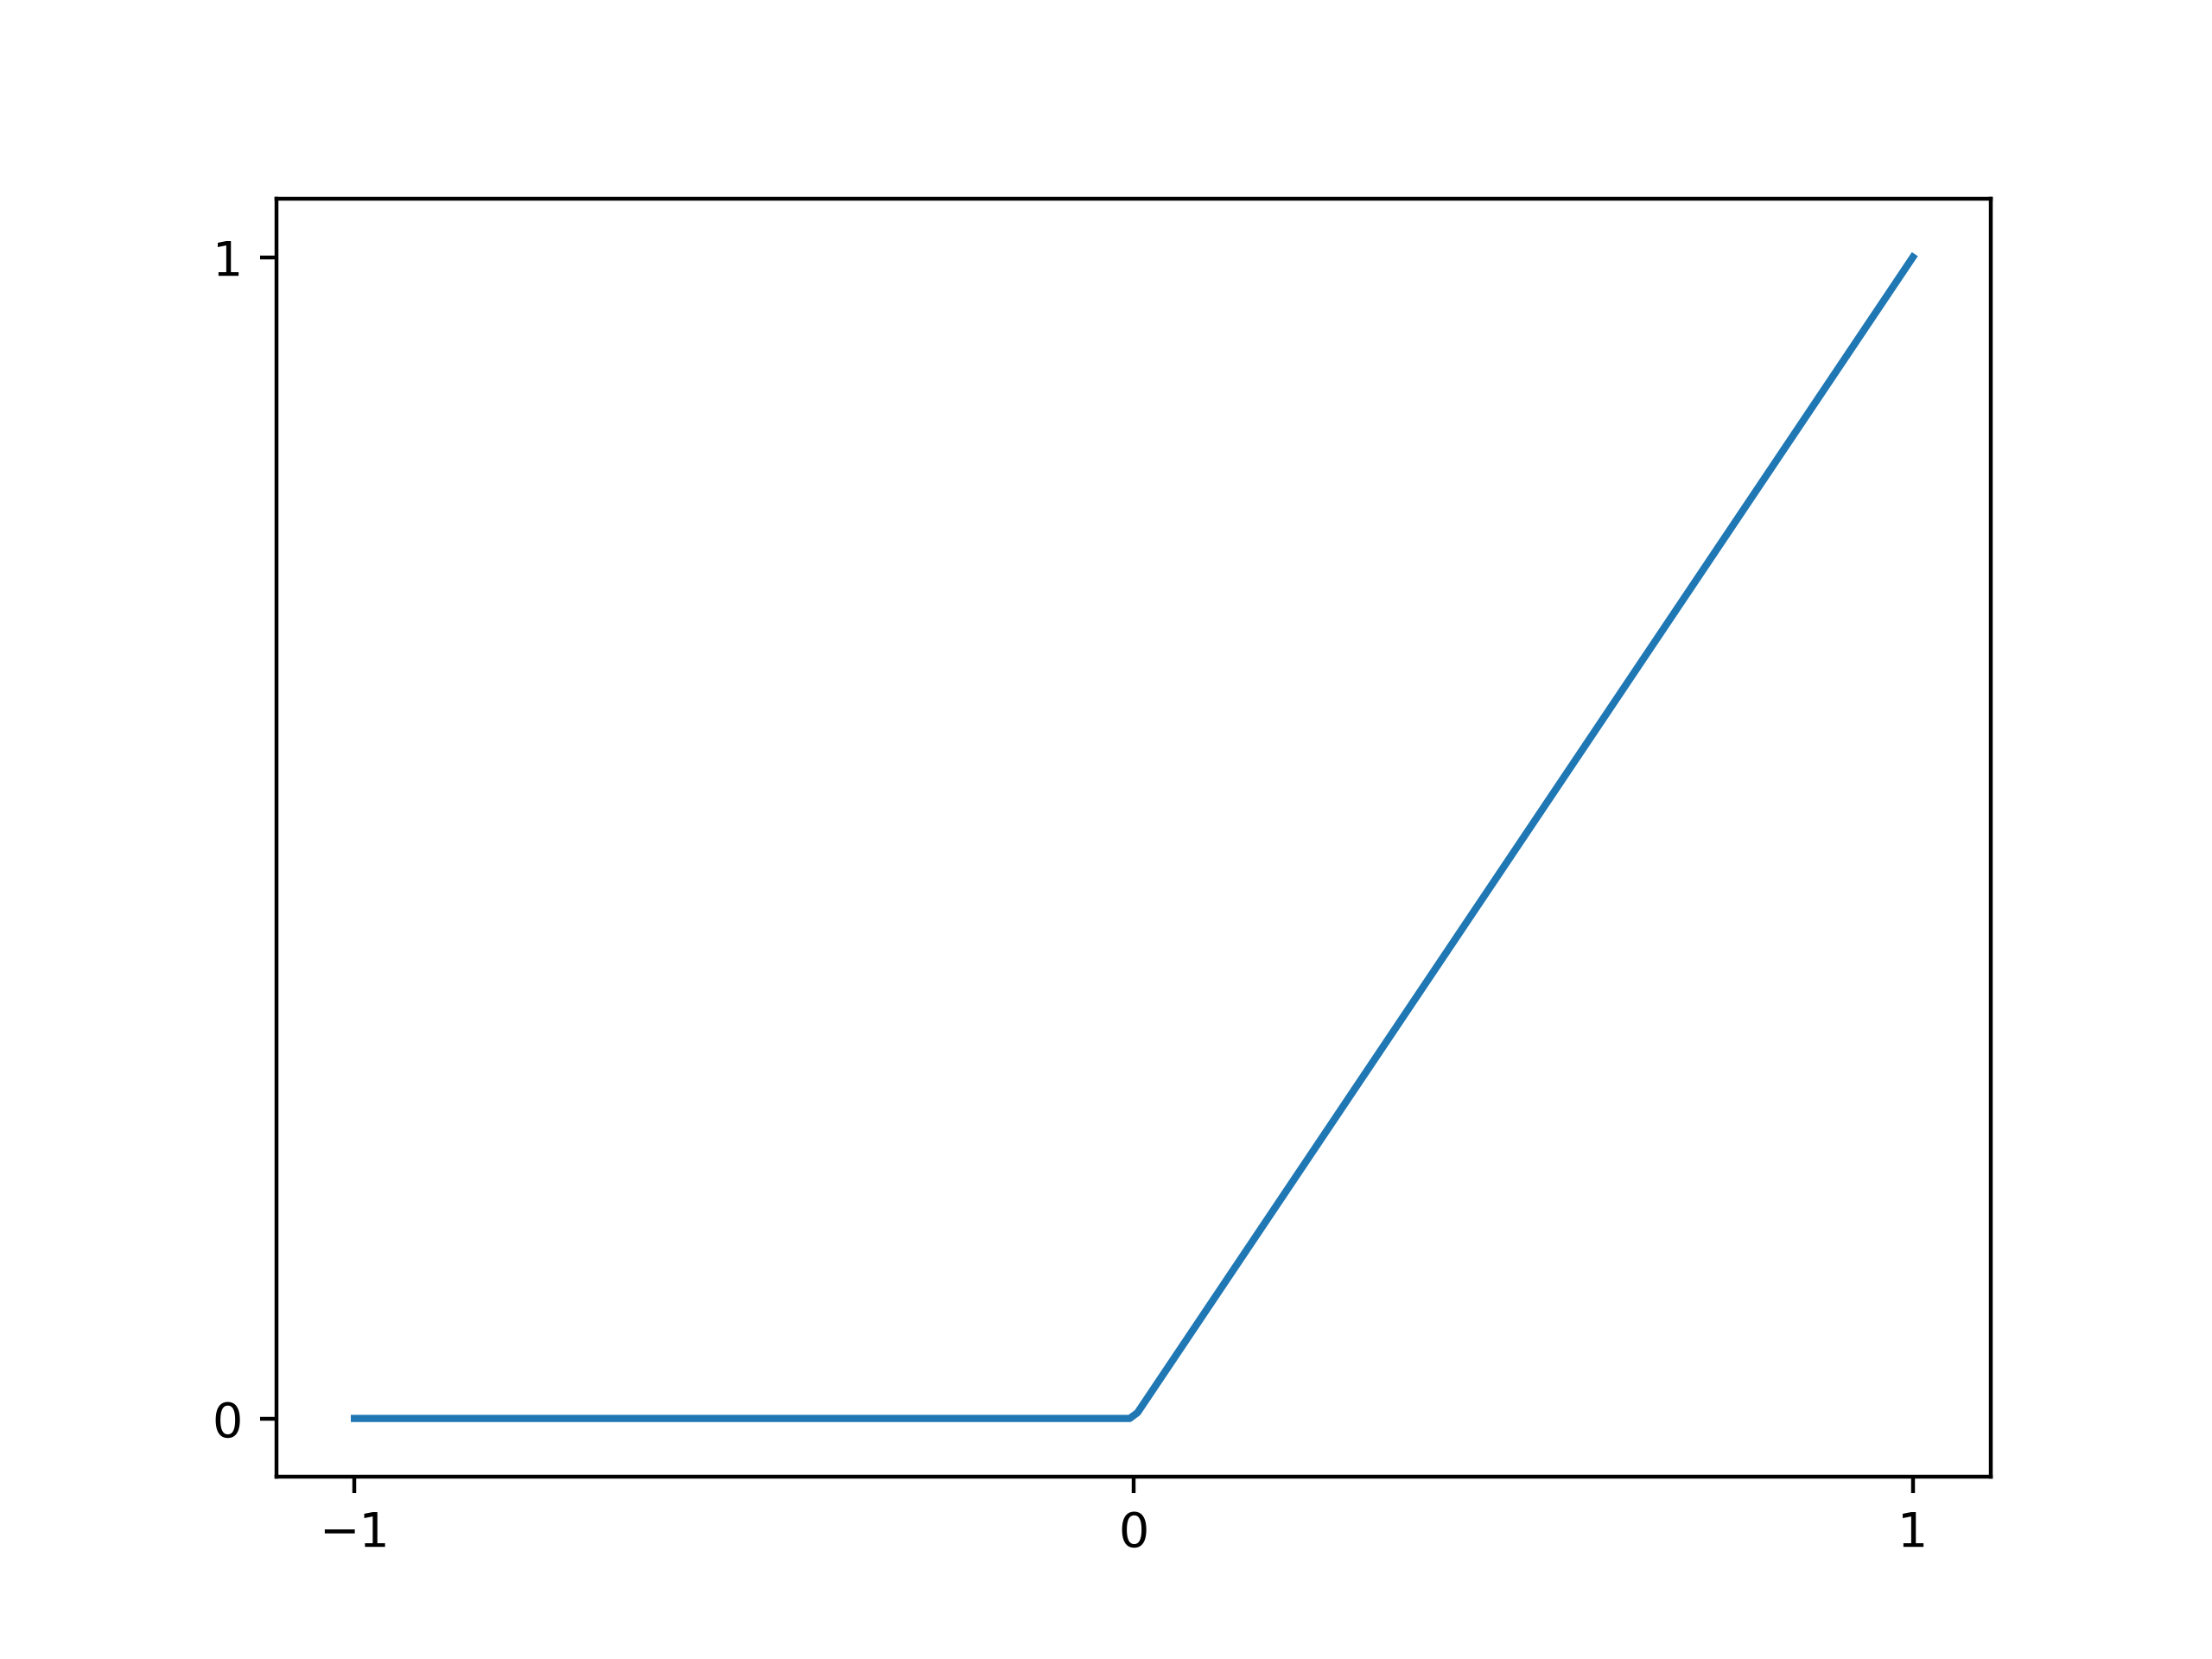
\includegraphics[width=0.3\textwidth]{relu.png} &
			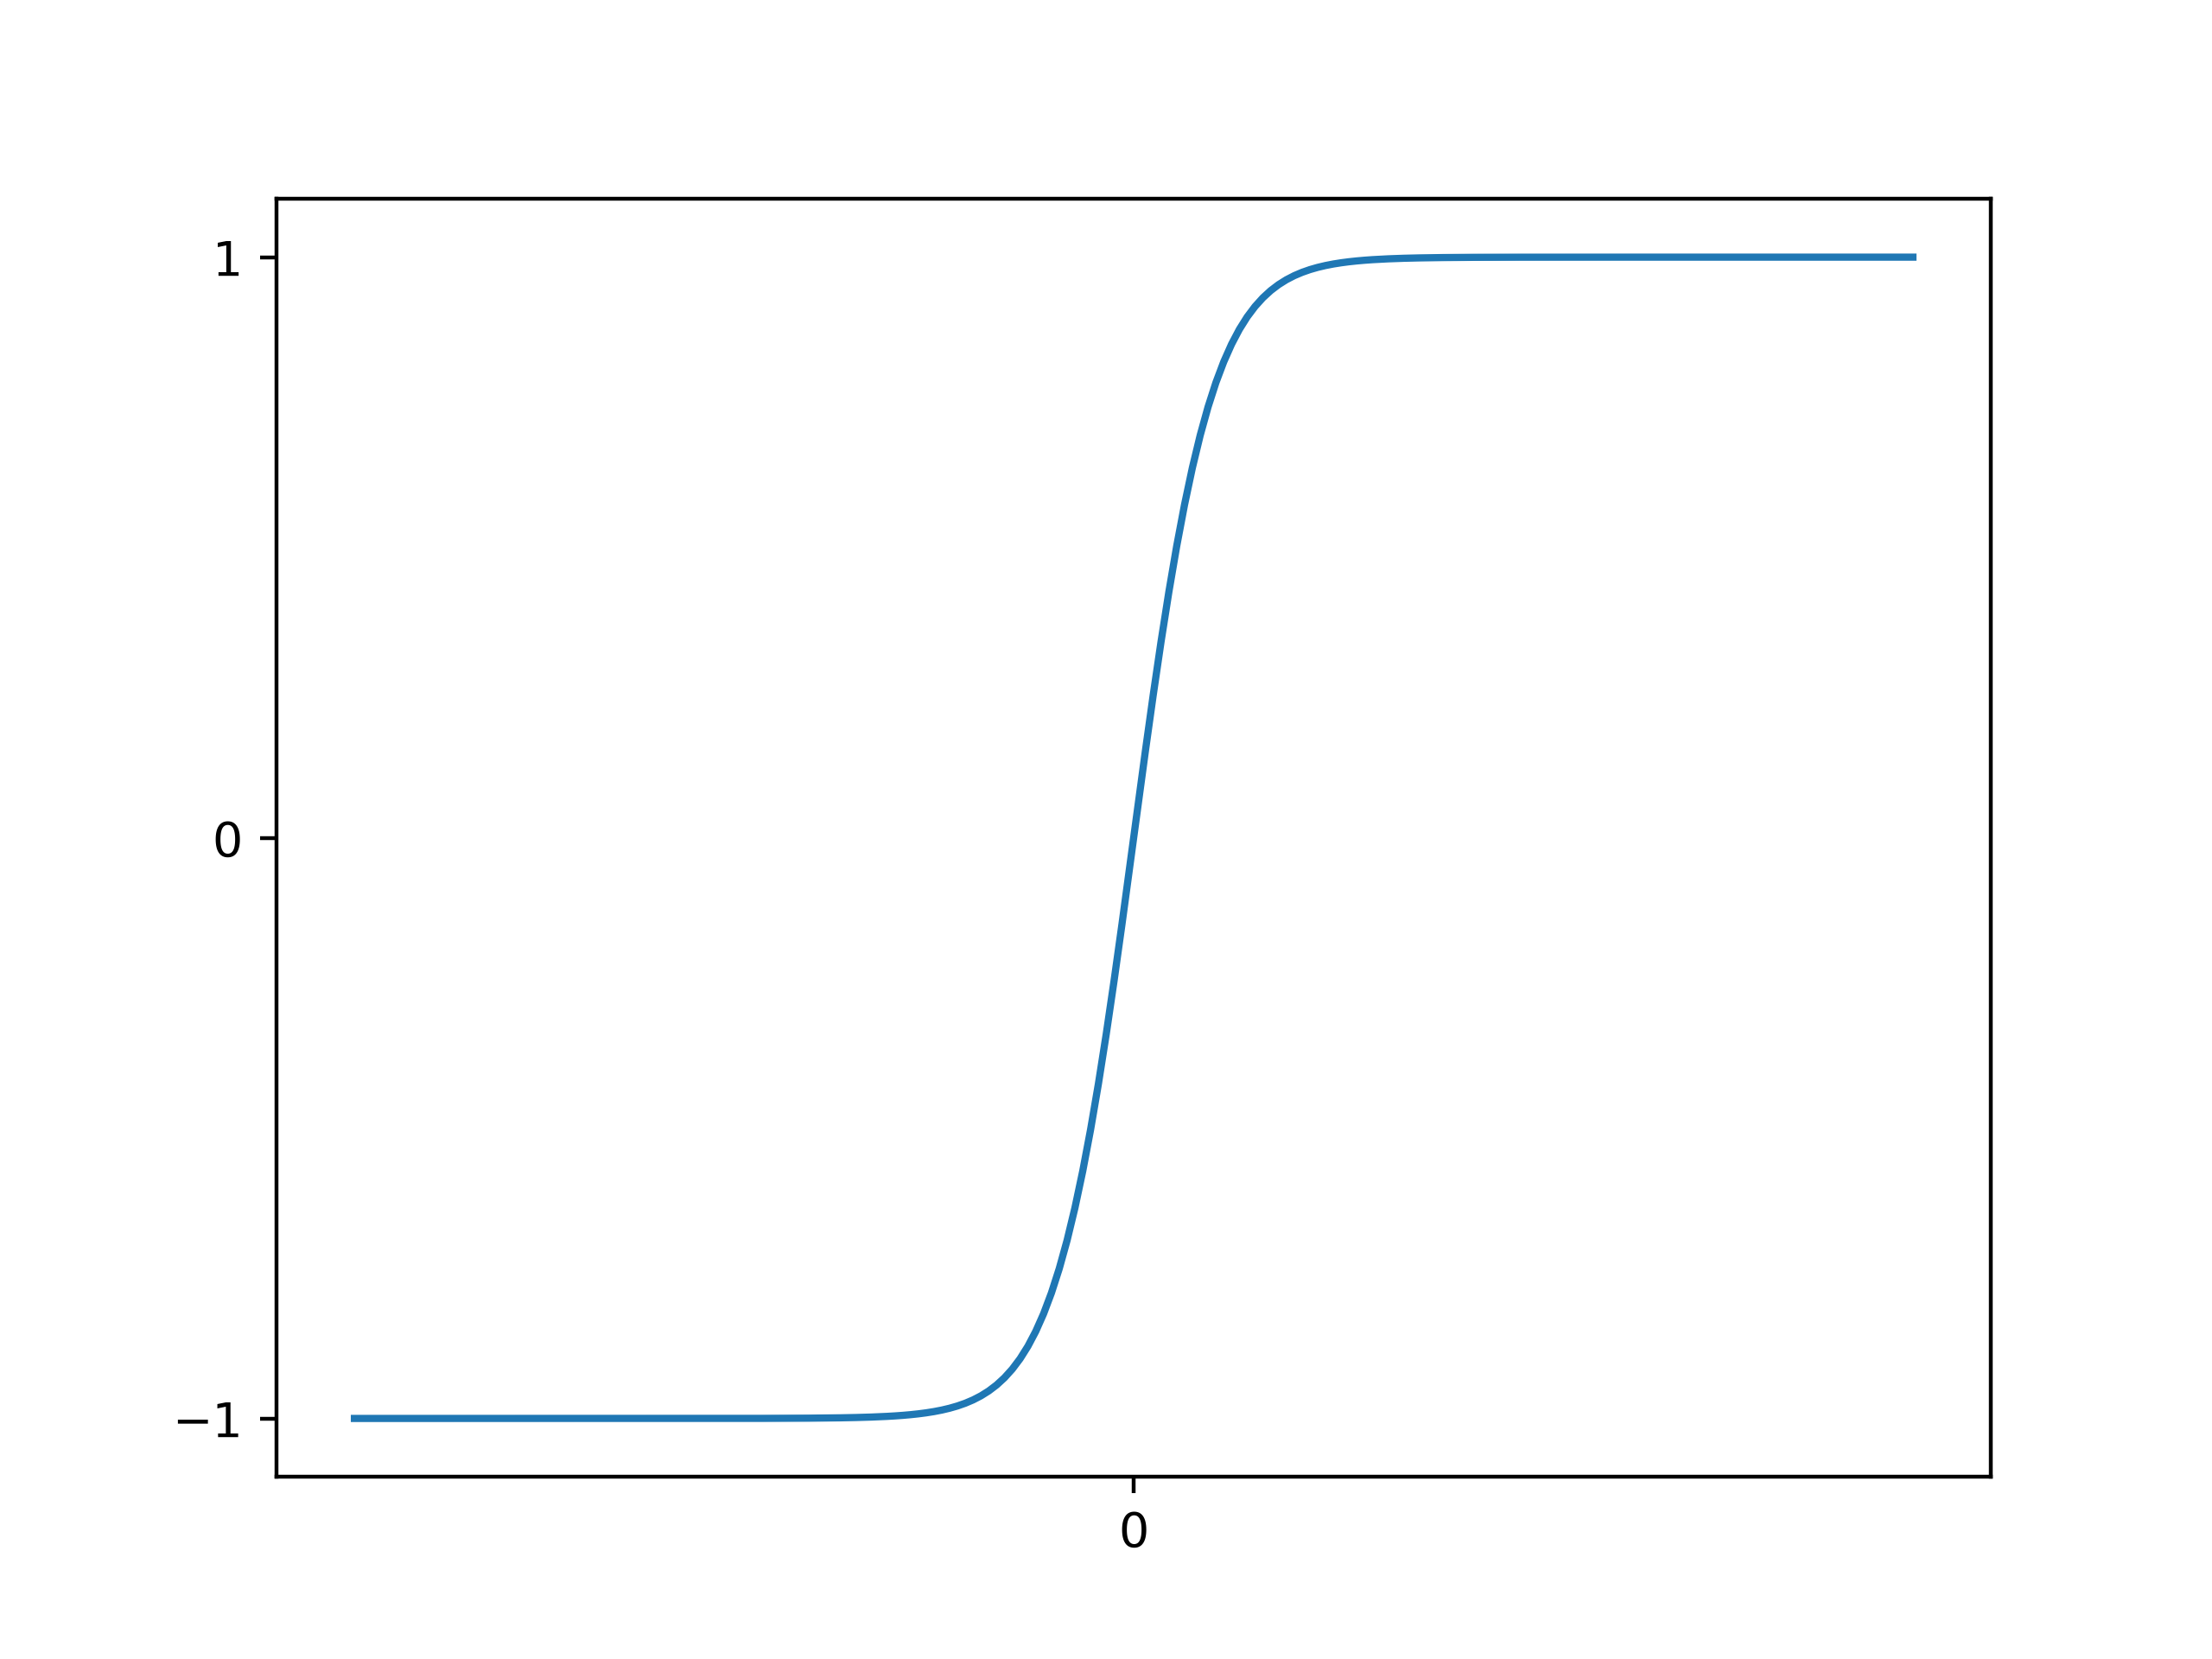
\includegraphics[width=0.3\textwidth]{tanh.png}       \\
			(a)                                             & (b)
		\end{tabular}
	\end{center}
	\caption{多图}
\end{figure}

\section{勾股定理的近代形式}

\begin{thm}[{\color{NavyBlue}\textbf{勾股定理}}]
	直角三角形斜边平方等于两腰平方和.
\end{thm}
\begin{lemma}[77]
	紧接定理编号
\end{lemma}

可用符号语言描述为:设直角三角形ABC,其中$\angle C=90^\circ$,则有
\begin{equation}%	equation环境
	AC^2+BC^2=AB^2.
\end{equation}
\begin{equation}
	\int_{a}^{b} f(x) \,\mathrm{d}x
\end{equation}

满足式(1)的整数称为\emph{勾股数},\emph{Number of Pythagorean shares} % 强调,改变字体
第1节说的毕达哥拉斯学派得到的三元数组就是勾股数.下列表给出了两组较小的勾股数:

\begin{table}[h]
	\center
	\begin{tabular}{ccc}%tabular环境,|rrr|表示表格有三列,
		\hline %产生横线
		直角边$a$ & 直角边$b$ & 斜边$c$ \\ %\\换行,每行内部用&隔开.
		\hline
		3         & 4         & 5       \\
		5         & 12        & 13      \\
		\hline
	\end{tabular}
	\caption{勾股数}
\end{table}

\section{自定义命令}

\[
	\norm{v_n-v_m}
\]
\[
	\dv{f}{x},\dv[n]{f}{x},\dv{}{x}
\]
\[
	\seq{x}
\]
\[
	\seq{y}
\]
\[
	\seq[1][m]{y}
\]
\[
	\seq[n][m]{y}
\]

$\BB \thetab$


\section{数学公式}
盒子:
\[
	\boxed{a^2+b^2=c^2} \quad
	c = \sqrt[2]{a^2 + b^2}
\]
箭头:
\[
	\xleftarrow{x+y+z}\quad\xrightarrow[x<y]{a+b+c} %\quad 生成空格
\]
\begin{equation*}
	\overline{m+n}
\end{equation*}

\begin{equation*}
	\underbrace{a_1+\ldots+a_n}_{m+n}
\end{equation*}

\begin{equation*}
	\overbrace{a_1+\ldots+a_n}^{m+n}
\end{equation*}

矩阵:
\begin{equation*}
	\begin{matrix}
		0 & 1 \\
		1 & 0
	\end{matrix}
	\qquad
	\begin{pmatrix}
		2 & 0 \\
		0 & 2
	\end{pmatrix}
	\qquad
	\begin{bmatrix}
		3 & 0 \\
		0 & 3
	\end{bmatrix}
	\qquad
	\begin{Bmatrix}
		4 & 0 \\
		0 & 4
	\end{Bmatrix}
	\qquad
	\begin{vmatrix}
		5 & 0 \\
		0 & 5
	\end{vmatrix}
	\qquad
	\begin{Vmatrix}
		6 & 0 \\
		0 & 6
	\end{Vmatrix}
\end{equation*}

\begin{equation*}
	\boldsymbol{A} = \begin{bmatrix}
		x_{11} & x_{12} & \ldots & x_{1n} \\
		x_{21} & x_{22} & \ldots & x_{2n} \\
		\vdots & \vdots & \ddots & \vdots \\
		x_{n1} & x_{n2} & \ldots & x_{nn}
	\end{bmatrix}
\end{equation*}

横,竖线(arydshln宏包)
\begin{equation*}
	\left(
	\begin{array}{c|ccc:c}
		a_{11} & a_{12} & \cdots & a_{1n} & b_1    \\
		\hline
		a_{21} & a_{22} & \cdots & a_{2n} & b_2    \\
		\hdashline
		\vdots & \vdots &        & \vdots & \vdots \\
		a_{m1} & a_{m2} & \cdots & a_{mn} & b_m
	\end{array}
	\right)
\end{equation*}

分块矩阵:

堆叠:
\begin{equation*}
	\sum_{\substack{0 < i < n \\ 0 < j < m}}p_{ij}
\end{equation*}
强制堆叠:$\max_{i>1} \rightarrow \max\limits_{i>1}$

数学环境空格:
\begin{equation*}
	x,y\qquad x,y,\quad x,y \quad x~y
\end{equation*}

分数:
$\frac{1}{2}$,$\tfrac{1}{2}$,$\cfrac{1}{2}$

\subsection{数学重音和上下括号}
\begin{equation}
	\bar{x_0} \quad \bar{x}_0 \quad \underline{x_0}
\end{equation}

\begin{equation}
	\vec{x_0} \quad \vec{x}_0 \quad \overrightarrow{AB}
\end{equation}

\begin{equation}
	\hat{\mathrm{e}} \quad \widehat{XY}a
\end{equation}

\subsection{多行公式}

对不需要对齐的长公式可以用multiline环境(无编号版本后带*),需要对齐的长公式可以用split环境
(称为次环境,因为必须包含在其他数学环境内)

multiline:
\begin{multline}
	a=b+c+d \\
	+e+f
\end{multline}

split:(按\&对齐)
\begin{equation}
	\begin{split}
		x = & a+b+c\\
		& d+e+f
	\end{split}
\end{equation}

\subsubsection{公式组}

不需要对齐的用gather环境,需要对齐的用align环境(均有无编号版本,后接*)

gather:
\begin{gather}
	a=b+c+d \\
	x=y+z  \notag %这一行不生成编号
\end{gather}

align:
\begin{align}
	a & = b+c+d \\
	x & = x+y
\end{align}

\begin{align*}
	a = b+c+ & d \\
	x = y  + & d % 是按&所在位置对齐
\end{align*}

\subsubsection{公式组合成块}
最常见的是case环境(次环境),它在几个公式前用花括号括起来,如

\begin{equation}\label{eq:Dirichlet}
	D(x) = \begin{cases}
		1, & \text{if}{~~} x \in \mathbb{Q};                   \\
		0, & \text{if}{~~} x \in \mathbb{R}\setminus\mathbb{Q}
	\end{cases}
\end{equation}
式\eqref{eq:Dirichlet}为Dirichlet函数.({\color{red}公式引用命令为eqref,而非ref})

mathtools宏包进一步提供了dcases环境,保证每行公式都是显示格式大小.
\[
	\left| x-\frac{1}{2}\right| = \begin{dcases}
		x-\frac{1}{2}, & x \geq \frac{1}{2}; \\
		\frac{1}{2}-x, & x < \frac{1}{2}.
	\end{dcases}
\]

更一般的情况,gathered环境把几行公式居中排列做为一个整体,如:
\[
	\left.
	\begin{gathered}
		S \subseteq T \\
		S \supseteq T
	\end{gathered}
	\right\}
	\implies S=T
\]

类似的,mathtools提供的lgathered,rgathered环境把几行公式向左(右)排列,做为一个整体.
\begin{equation}
	\text{比较曲线}
	\left\{
	\begin{lgathered}
		x = \sin y , y = \cos x \\
		x = t + \sin t , y = \cos t
	\end{lgathered}
	\right.
\end{equation}

\begin{equation}
	\left.
	\begin{rgathered}
		x = \sin y , y = \cos x \\
		x = t + \sin t , y = \cos t
	\end{rgathered}
	\right\}\text{比较曲线}
\end{equation}

每个公式单独编号,需要cases宏包(numcases环境)
\begin{numcases}{f(x)=}
	a+b,& 0 \\
	c+d,& 1
\end{numcases}

子公式编号
\begin{subequations}\label{eq:par}
	\begin{align}
		a & = b \label{eq:a} \\
		c & = d \label{eq:b}
	\end{align}
\end{subequations}
公式\eqref{eq:par}的子公式编号\eqref{eq:a}和\eqref{eq:b}.

\subsubsection{数学字体}
\begin{itemize}
	\item $\mathrm{ABCDabcd 1234}$(直体,数学环境字母为斜体,但算子应为直体,如$\mathrm{d}x$) mathrm;
	\item $\mathcal{ABCD}$ \\mathcal;
	\item $\mathscr{ABCD}$ \\mathscr (mathrsfs宏包)
	\item $\mathfrak{ABCD}$ \\mathfrak (amssymb)
	\item $\mathbb{ABCD}$ \\mathbb (amssymb)
	\item 数学粗体$\boldsymbol{A},\boldsymbol{f},\boldsymbol{n},\boldsymbol{\theta}
	      $(数学粗体$\mathbf{x},\mathbf{f}$一般不用)
	\item 非数学环境粗体: \textbf{非数学环境}
\end{itemize}

\section{tcolor宏包}
\begin{tcolorbox}
	test
\end{tcolorbox}

\begin{tcolorbox}
	\begin{thm}[\textbf{勾股定理}]
		$a^2+b^2=c^2$
	\end{thm}
\end{tcolorbox}

\subsection{配色}
须在tcolorbox宏包前先引入xcolor的dvipsnames
\begin{quote}
	usepackage[dvipsnames]\{xcolor\}
\end{quote}
\begin{tcolorbox}[colback=Emerald!10,colframe=cyan!40!black,title=\textbf{配色1}]
	配色
\end{tcolorbox}

\begin{tcolorbox}[colback=JungleGreen!10!Cerulean!15,colframe=CornflowerBlue!60!Black,title=\textbf{配色2}]
	配色
\end{tcolorbox}

\begin{tcolorbox}[title=\textbf{配色3},colback=SeaGreen!10!CornflowerBlue!10,colframe=RoyalPurple!55!Aquamarine!100!]
	配色
\end{tcolorbox}

\begin{tcolorbox}[title=\textbf{配色4}, colback=Salmon!20, colframe=Salmon!90!Black]
	配色
\end{tcolorbox}

\subsection{定理环境}
tcolor宏包提供了theorems 程序包来实现定理类的环境

\begin{lstlisting}
	\newtcbtheorem[init options]{name}{display name}{options}{prefix}
\end{lstlisting}

\begin{mytheo}{勾股定理}{}\label{thm:1}
	$a^2+b^2=c^2$
\end{mytheo}
引用定理\ref{thm:1}

\begin{mylemma}{引理}{lemma:1}
	引理
\end{mylemma}
\begin{mydef}{}{}
	定义
\end{mydef}

\section{代码环境}
\begin{lstlisting}[language=Python,keywordstyle=\bfseries\color{NavyBlue},basicstyle=\ttfamily]
	import math
	import numpy as np
\end{lstlisting}

\section{图表}
插图一般置于浮动环境figure中,表一般置于浮动环境table中.\\
浮动环境位置参数:
\begin{itemize}
	\item[h:]表示here
	\item[t:]表示top
	\item[b:]表示bottom1
	\item[p:]表示单独一页
\end{itemize}
四个参数组合,如[ht]表示允许浮动体出现在here(环境所在位置)和顶部.

\subsection{列表}

\textbf{常规列表}
\begin{itemize}
	\item[*] 第一条
		\item[x]第二条
		\subitem[aa]第三条
\end{itemize}

\textbf{有序列表}
\begin{enumerate}
	\item 第一条
	      \subitem 第二条
	\item 第三条
\end{enumerate}

不同编号(enumerate宏包)
\begin{enumerate}[(1)]
	\item 第一条
	\item 第三条
\end{enumerate}

\begin{enumerate}[1)]
	\item 第一条
	\item 第三条
\end{enumerate}

\begin{enumerate}[(a)]
	\item 第一条
	\item 第三条
\end{enumerate}

\begin{enumerate}[i.]
	\item 第一条
	\item 第三条
\end{enumerate}

\begin{enumerate}[step1]
	\item 第一条
	\item 第三条
\end{enumerate}

\subsection{图}
需要宏包graphicx,命令为includegraphics[scale= , width=,height=]\{插图名\} \\
scale:图片缩放倍数

\begin{figure}[htbp] % h:表示here,可选t:top等
	\center %居中命令
	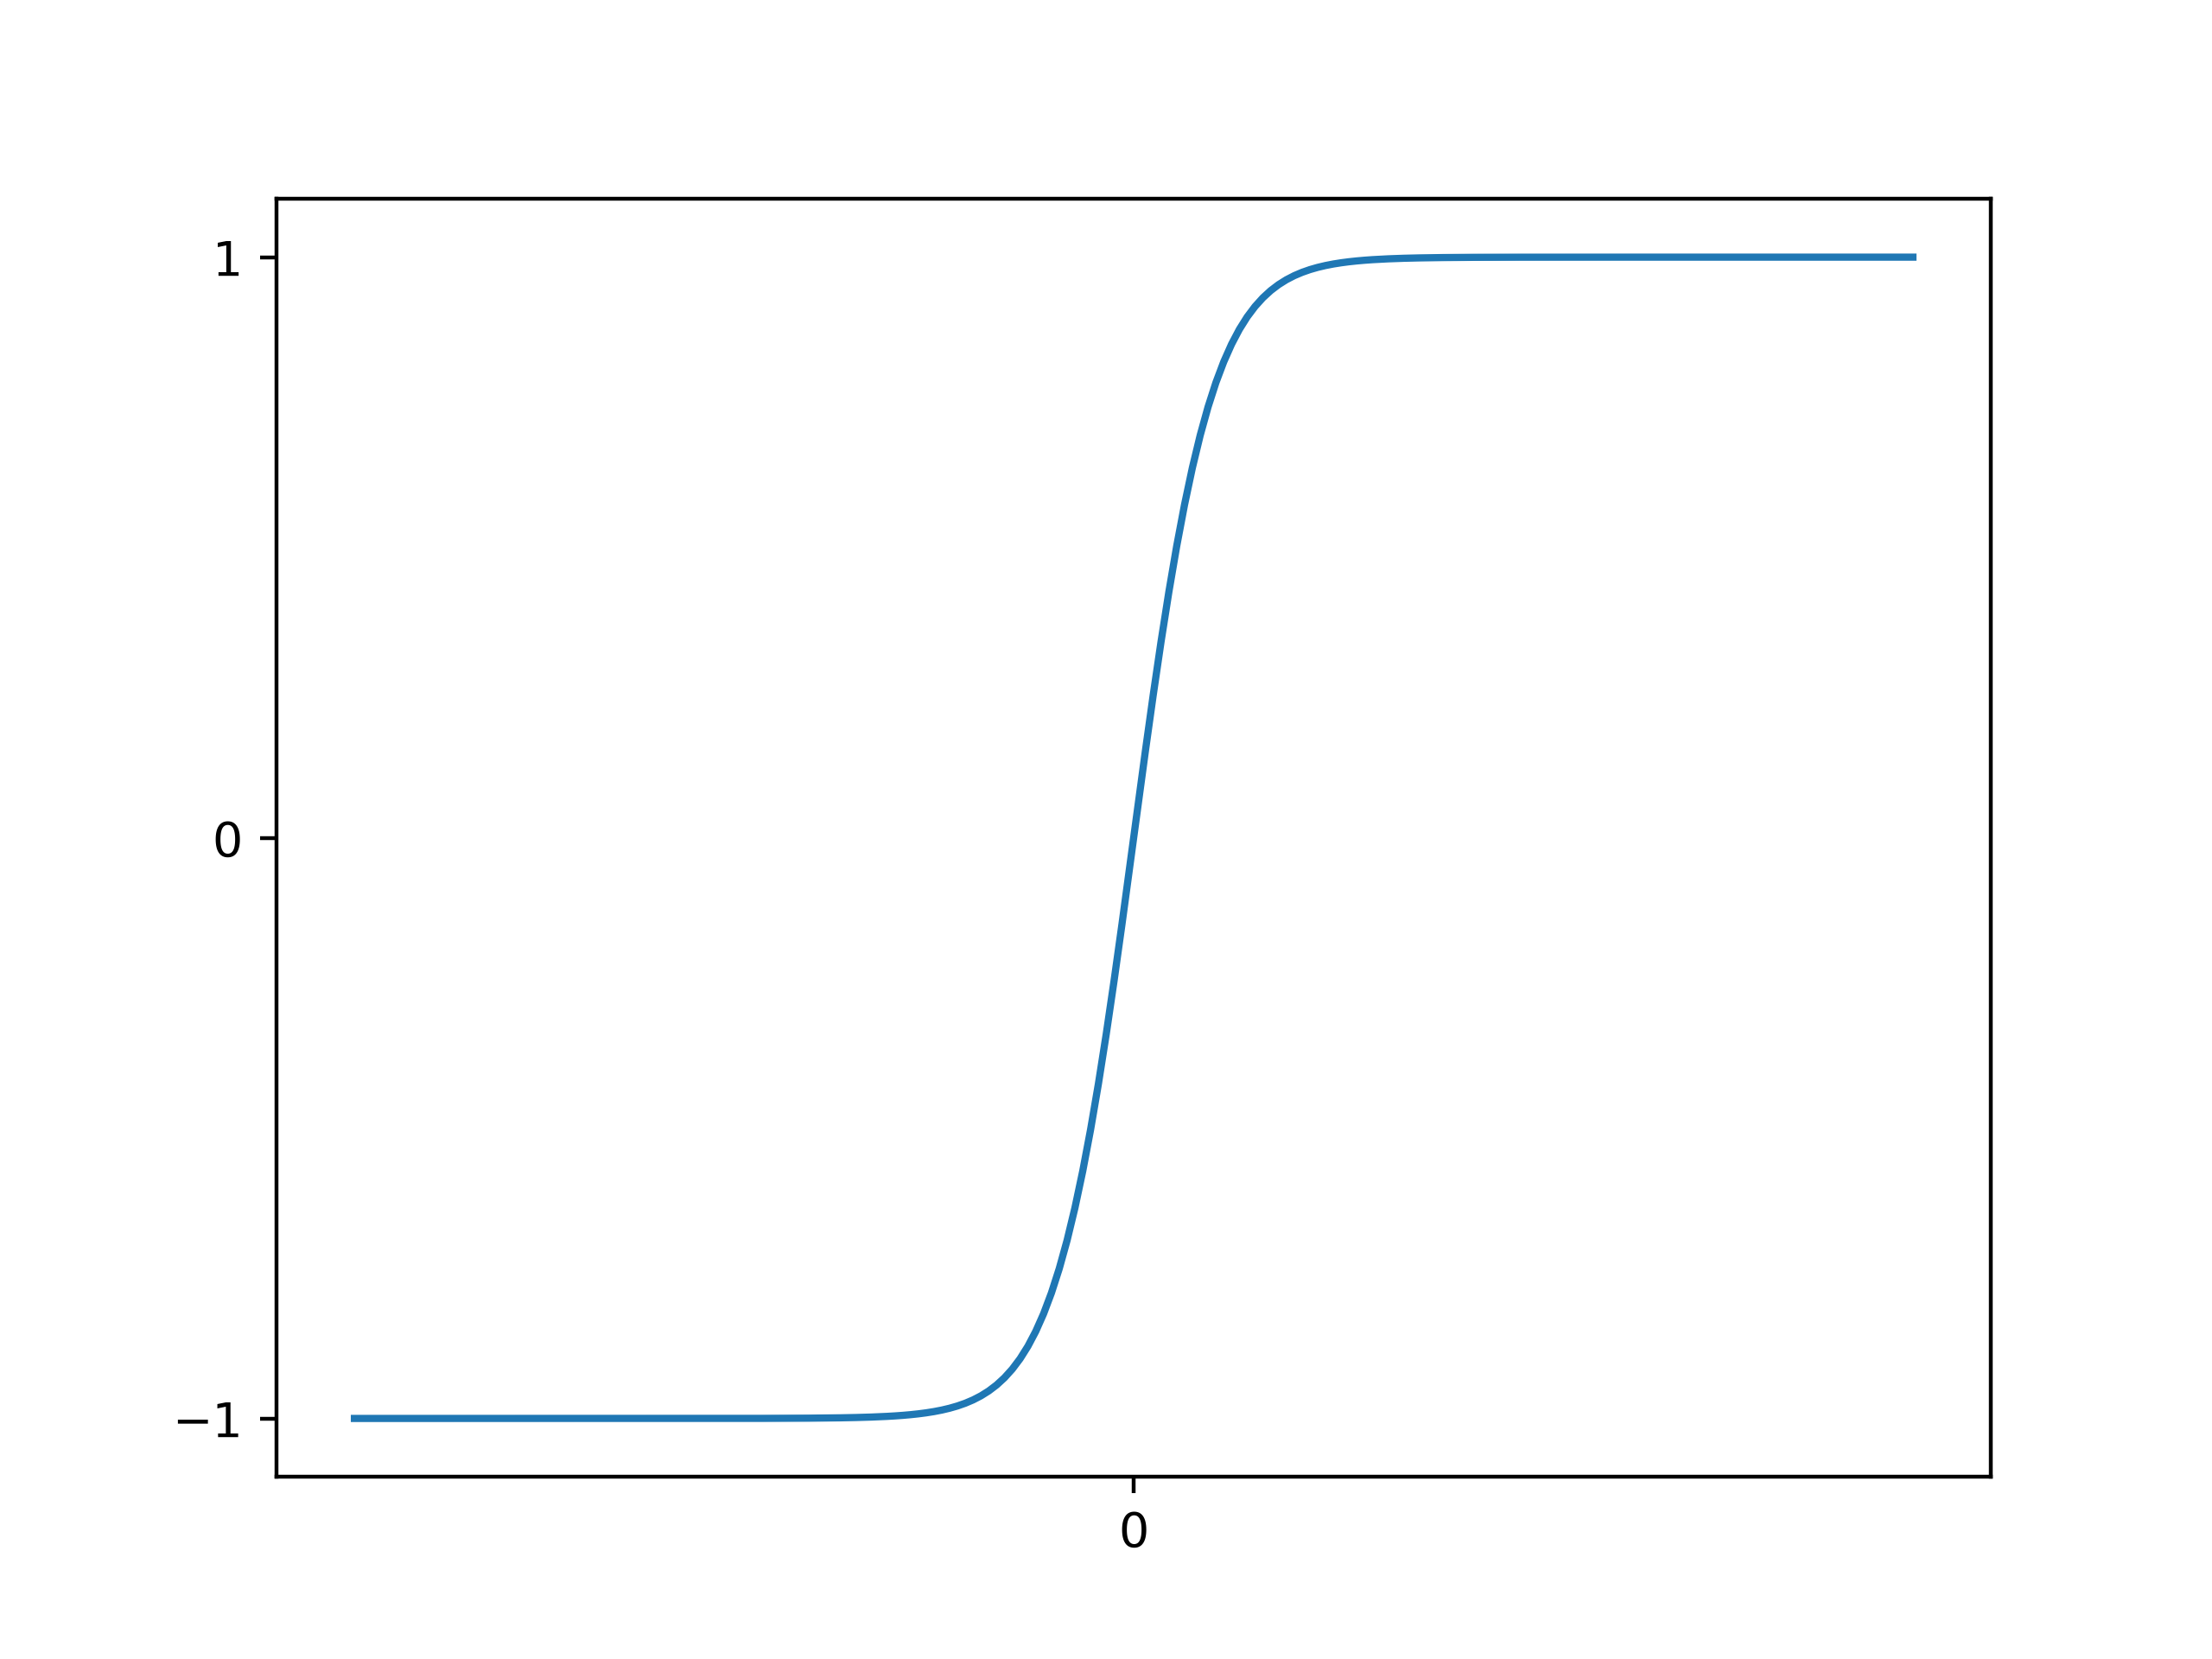
\includegraphics[scale=0.5]{tanh.png}
	\caption{标题在下} %标题
\end{figure}

\begin{figure}[htbp] % h:表示here,可选t:top等
	\center %居中命令
	\caption{标题在上} %标题
	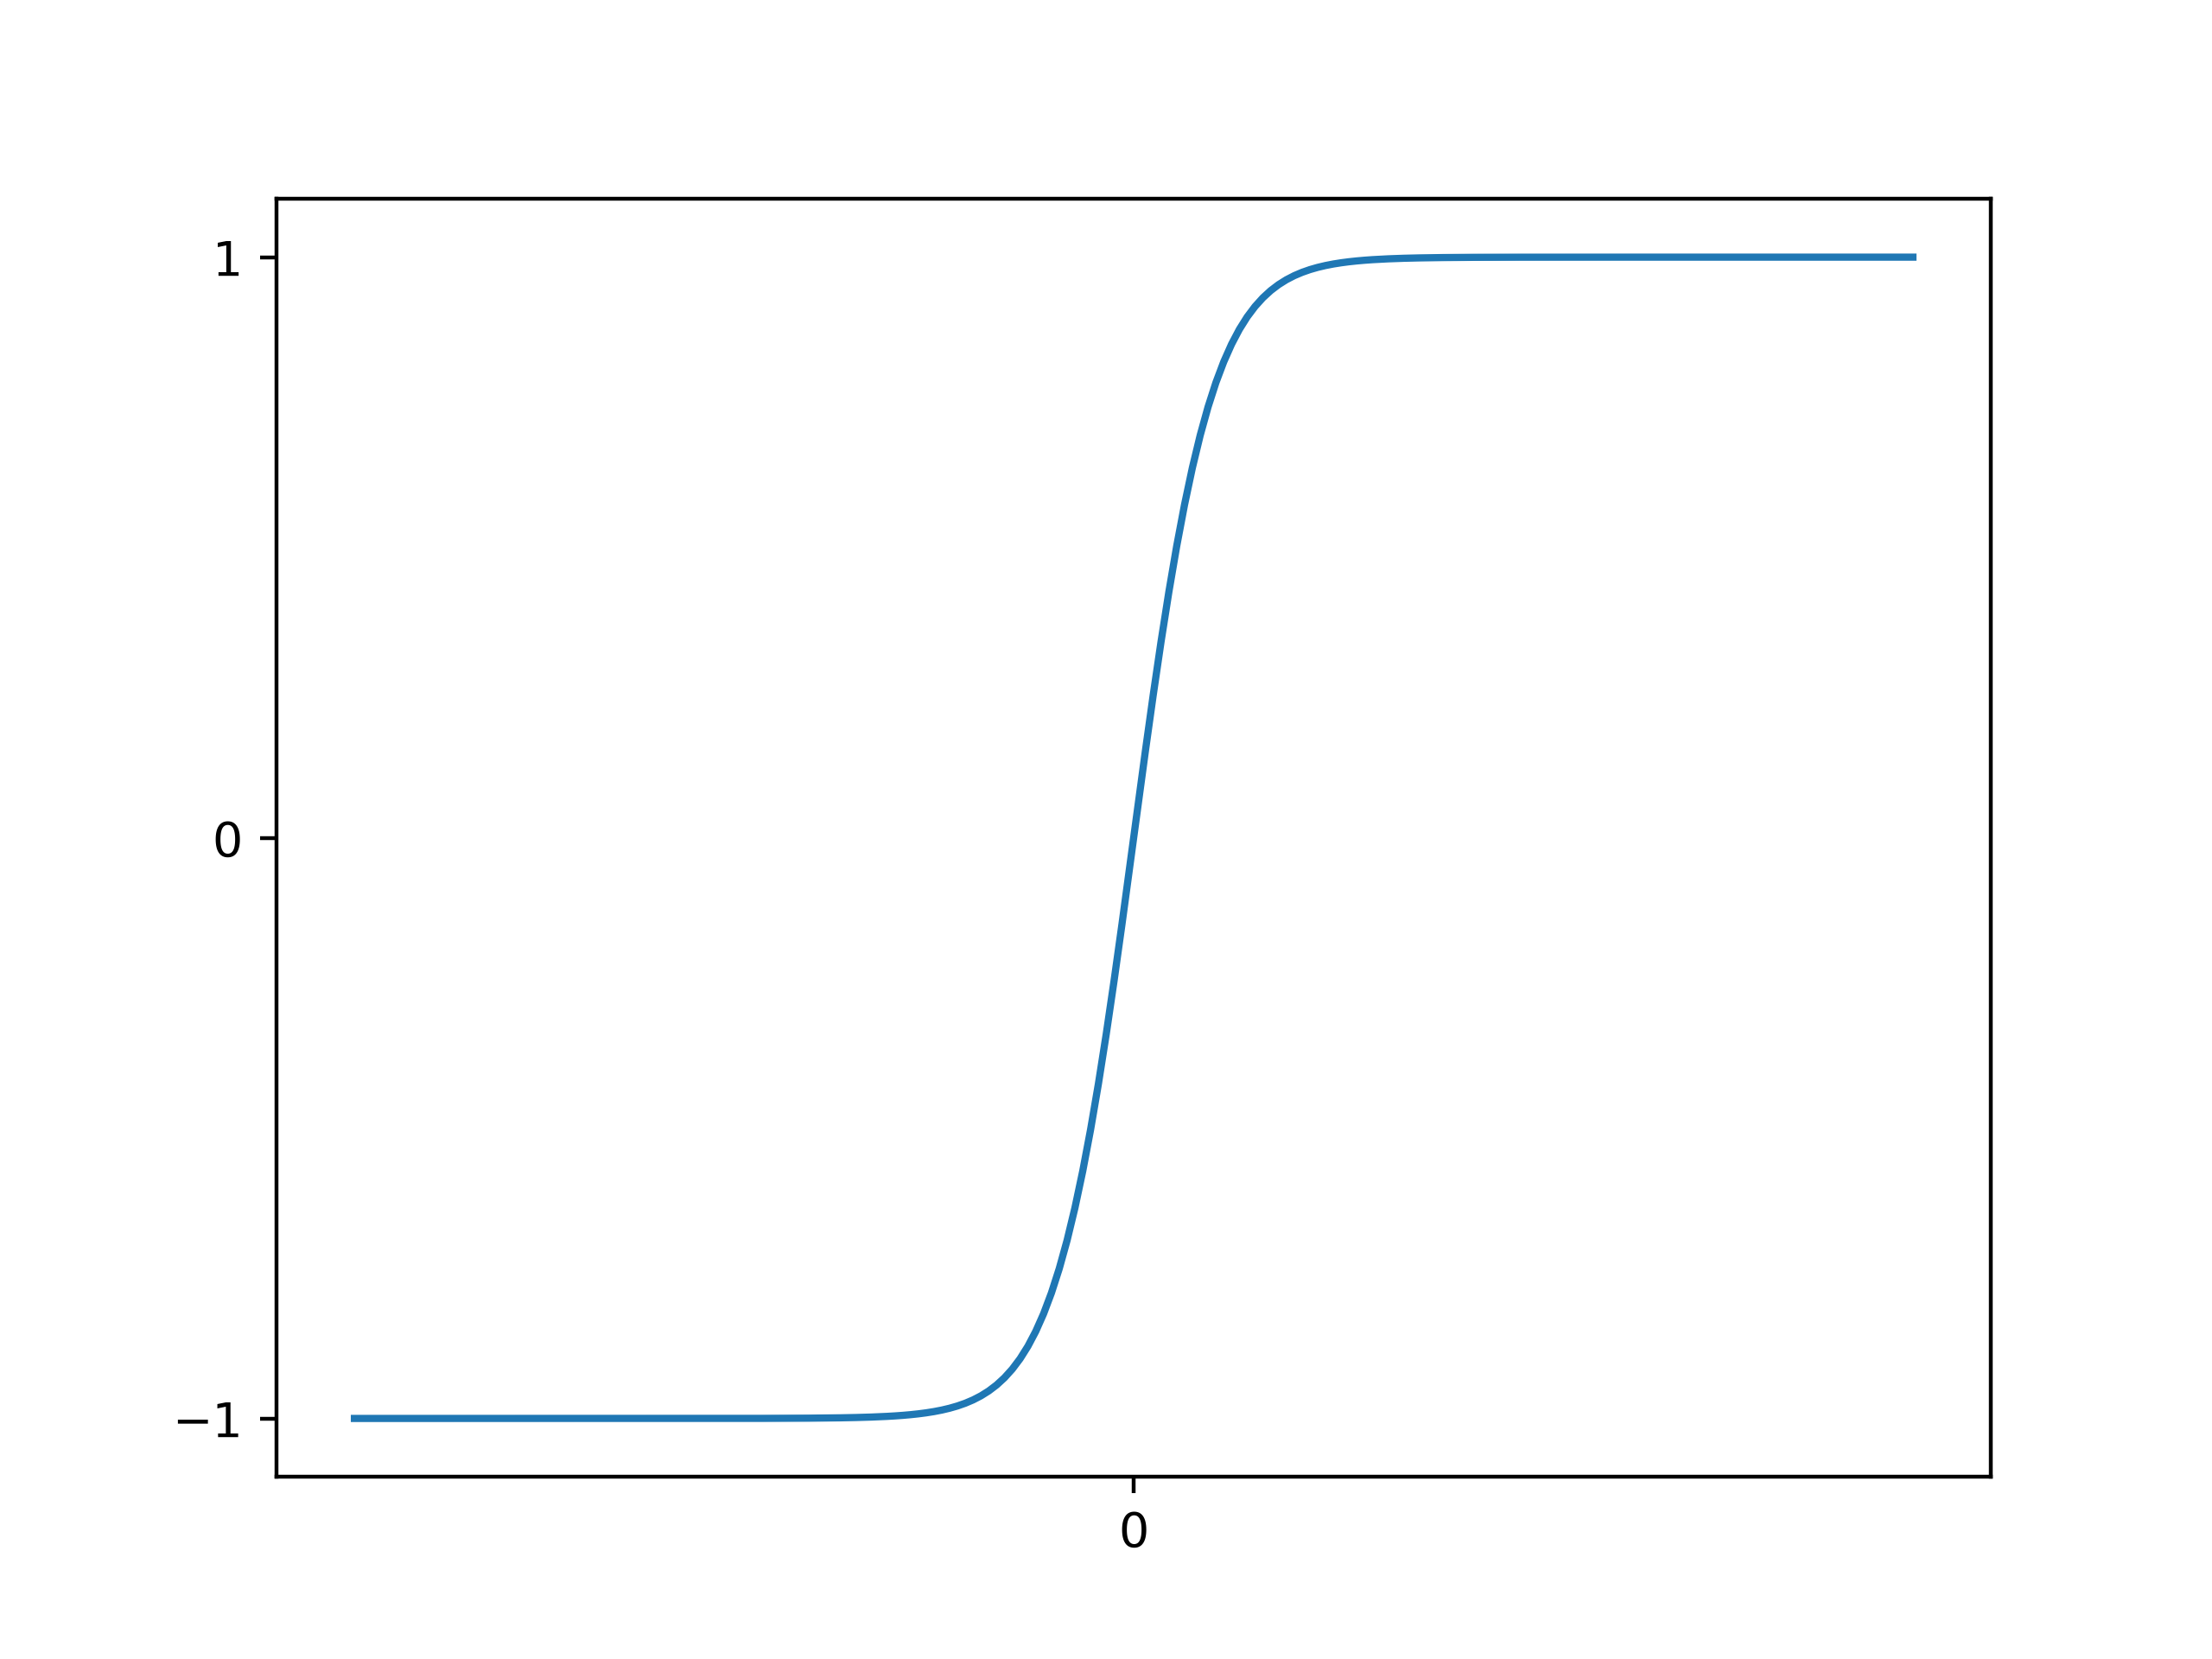
\includegraphics[scale=0.5]{tanh.png}
\end{figure}

\subsection{表}
\subsubsection{三线表}
需要宏包booktabs,lll表示三列,l(left)表示左对齐,可选c(center),r(right)
\begin{table}[htbp]
	\center
	\begin{tabular}{lll}
		\toprule
		\toprule
		1 & 2 & 3 \\
		\midrule
		4 & 5 & 6 \\
		\bottomrule
	\end{tabular}
\end{table}

\subsubsection{表格宽度}
控制某栏宽度,可以将对齐方式参数l,c,r改为p(宽度)
\begin{table}[htbp]
	\caption{控制表格宽度}
	\center
	\begin{tabular}{p{100pt}p{100pt}p{100pt}}
		\toprule
		操作系统  & 发行版  & 编辑器    \\
		\midrule
		Windows   & MikTeX  & Texstudio \\
		UnixLinux & TexLive & Vim       \\
		Mac OS    & MacTex  & Texshop   \\
		\bottomrule
	\end{tabular}
\end{table}

\subsubsection{跨列表格}
某栏需要横跨几列,可以使用multicolumn命令,它的前两个参数指定横跨的列数和对齐方式,
booktabs宏包的cmidrule命令用于横跨几列的横线.
\begin{table}[htbp]
	\caption{跨列表格}
	\center
	\begin{tabular}{lll}
		\toprule
		         & \multicolumn{2}{c}{常用工具}             \\ %第一列为空,接着横跨两列
		\cmidrule{2-3} %2-3列加下横线
		操作系统 & 发行版                       & 编辑器    \\
		\midrule
		Windows  & MikTeX                       & Texstudio \\
		Linux    & TexLive                      & Vim       \\
		Mac OS   & MacTex                       & Texshop   \\
		\bottomrule
	\end{tabular}
\end{table}

\subsubsection{跨行表格}
需要multirow宏包,multirow命令前两个参数是竖跨的行数和宽度
\begin{table}[htbp]
	\caption{跨行表格}
	\center
	\begin{tabular}{lllc}
		\toprule
		操作系统 & 发行版  & 编辑器    & \LaTeX                            \\
		\midrule
		Windows  & MikTeX  & Texstudio & \multirow{3}{100pt}{hello \LaTeX} \\
		\cline{2-3} % 同\cmidrule
		Linux    & TexLive & Vim                                           \\
		Mac OS   & MacTex  & Texshop                                       \\
		\bottomrule
	\end{tabular}
\end{table}

\begin{table}
	\center
	\caption{复杂点的表格}
	\begin{tabular}{cccccc}
		\toprule
		\multirow{2}{*}{训练过程} & \multicolumn{2}{c}{$K-NN$} & \multicolumn{2}{c}{优化} & \multirow{2}{*}{RMSLE}                          \\
		\cmidrule(r){2-3} \cmidrule(r){4-5}
		                          & 最优k                      & RMSLE                    & 最优$ \lambda $        & RMSLE                  \\
		\midrule
		$100000$                  & 16                         & 0.3243                   & le3                    & 0.3595 & \XSolidBrush  \\
		10000                     & 11                         & 0.3636                   & le3                    & 0.3775 & \Checkmark    \\
		1000                      & 7                          & 0.4296                   & le3                    & 0.4019 & \SixStar      \\
		100                       & 6                          & 0.5556                   & le3                    & 0.4019 & \JackStarBold \\
		\bottomrule
	\end{tabular}

\end{table}

\cleardoublepage

\subsubsection{diagbox}
需要宏包diagbox
\begin{table}
	\centering
	\begin{tabular}{cccc}
		\toprule
		\diagbox{\#layers}{\#neurons} & 10                  & 20                  & 30                  \\
		\midrule
		2                             & 5.76$\times10^{-2}$ & 2.33$\times10^{-2}$ & 9.23$\times10^{-3}$ \\
		4                             & 8.91$\times10^{-3}$ & 2.72$\times10^{-3}$ & 6.71$\times10^{-4}$ \\
		6                             & 2.97$\times10^{-3}$ & 2.50$\times10^{-4}$ & 2.32$\times10^{-4}$ \\
		\bottomrule
	\end{tabular}
	\caption{跳跃连接的{\rm IFNN}在不同隐藏层数{\rm (\#layers)}和每层神经元数{\rm (\#neurons)}的条件下,预测解的相对$\mathbb{L}_2$误差.}
\end{table}

\section{并列的图表}
直接把图表放在一个表格的浮动环境里

\begin{table}[h]
	\center
	\begin{tabular}{|c|c|}
		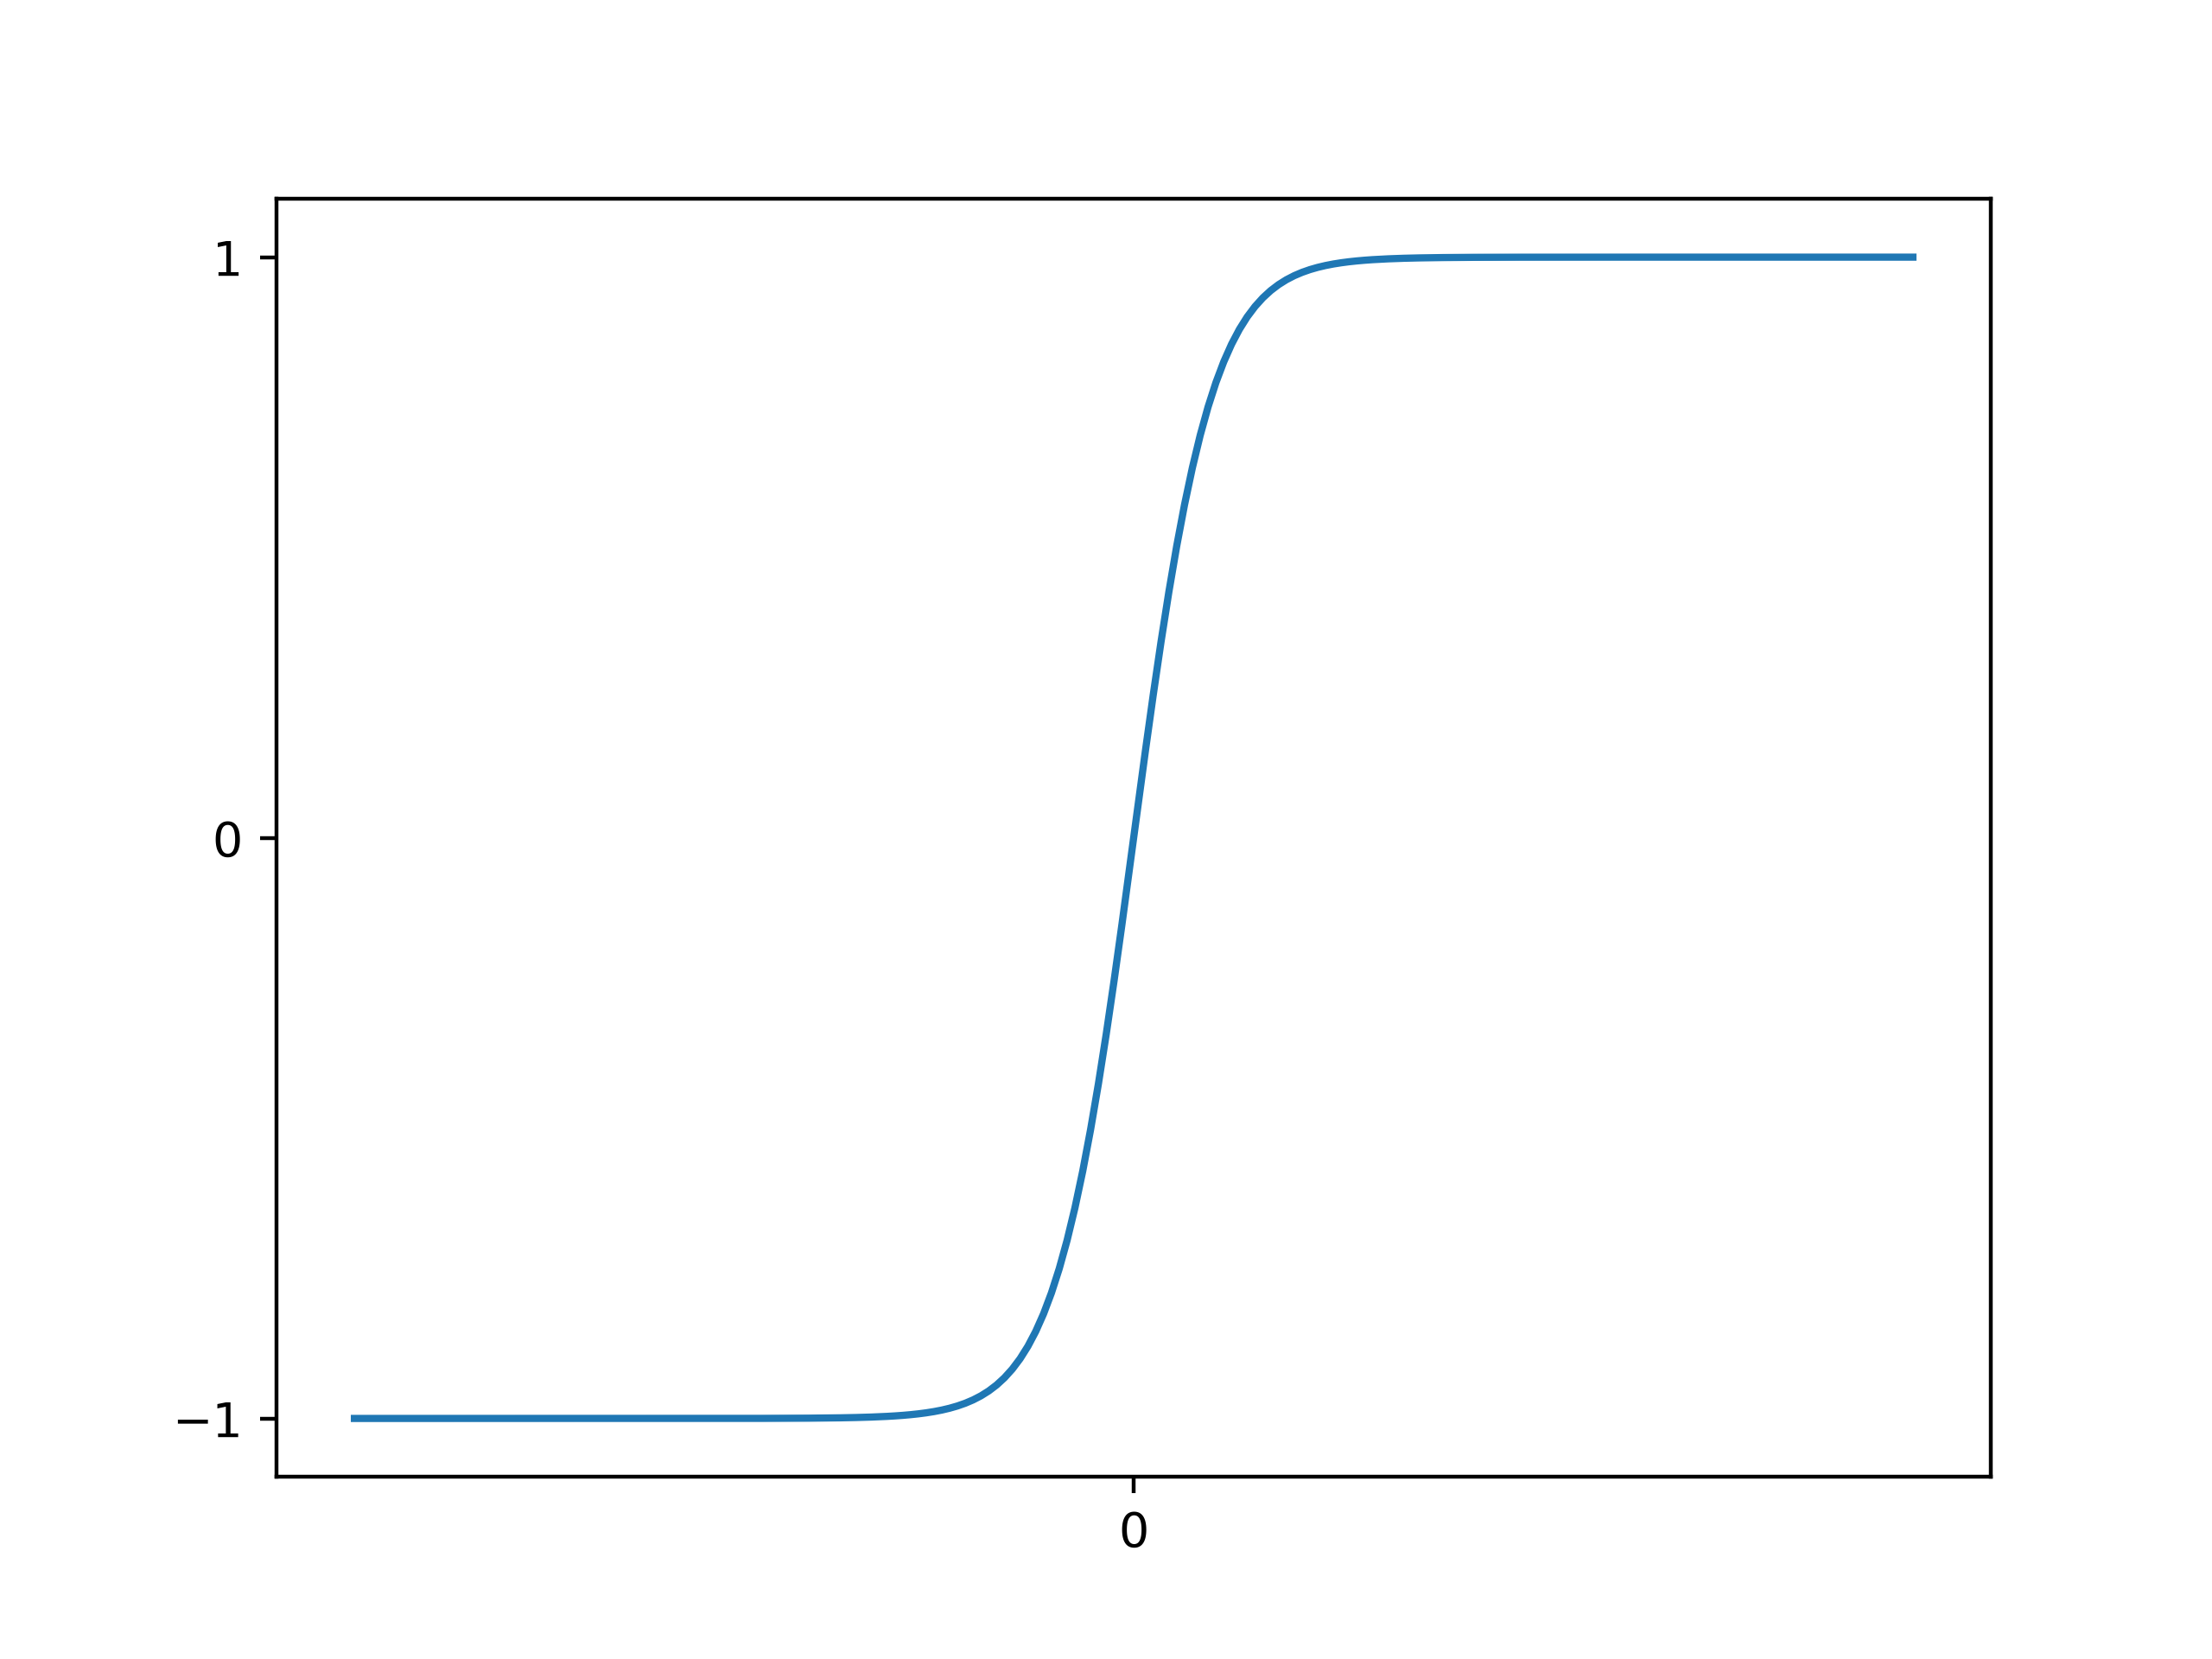
\includegraphics[scale=0.5]{tanh.png}
		 &
		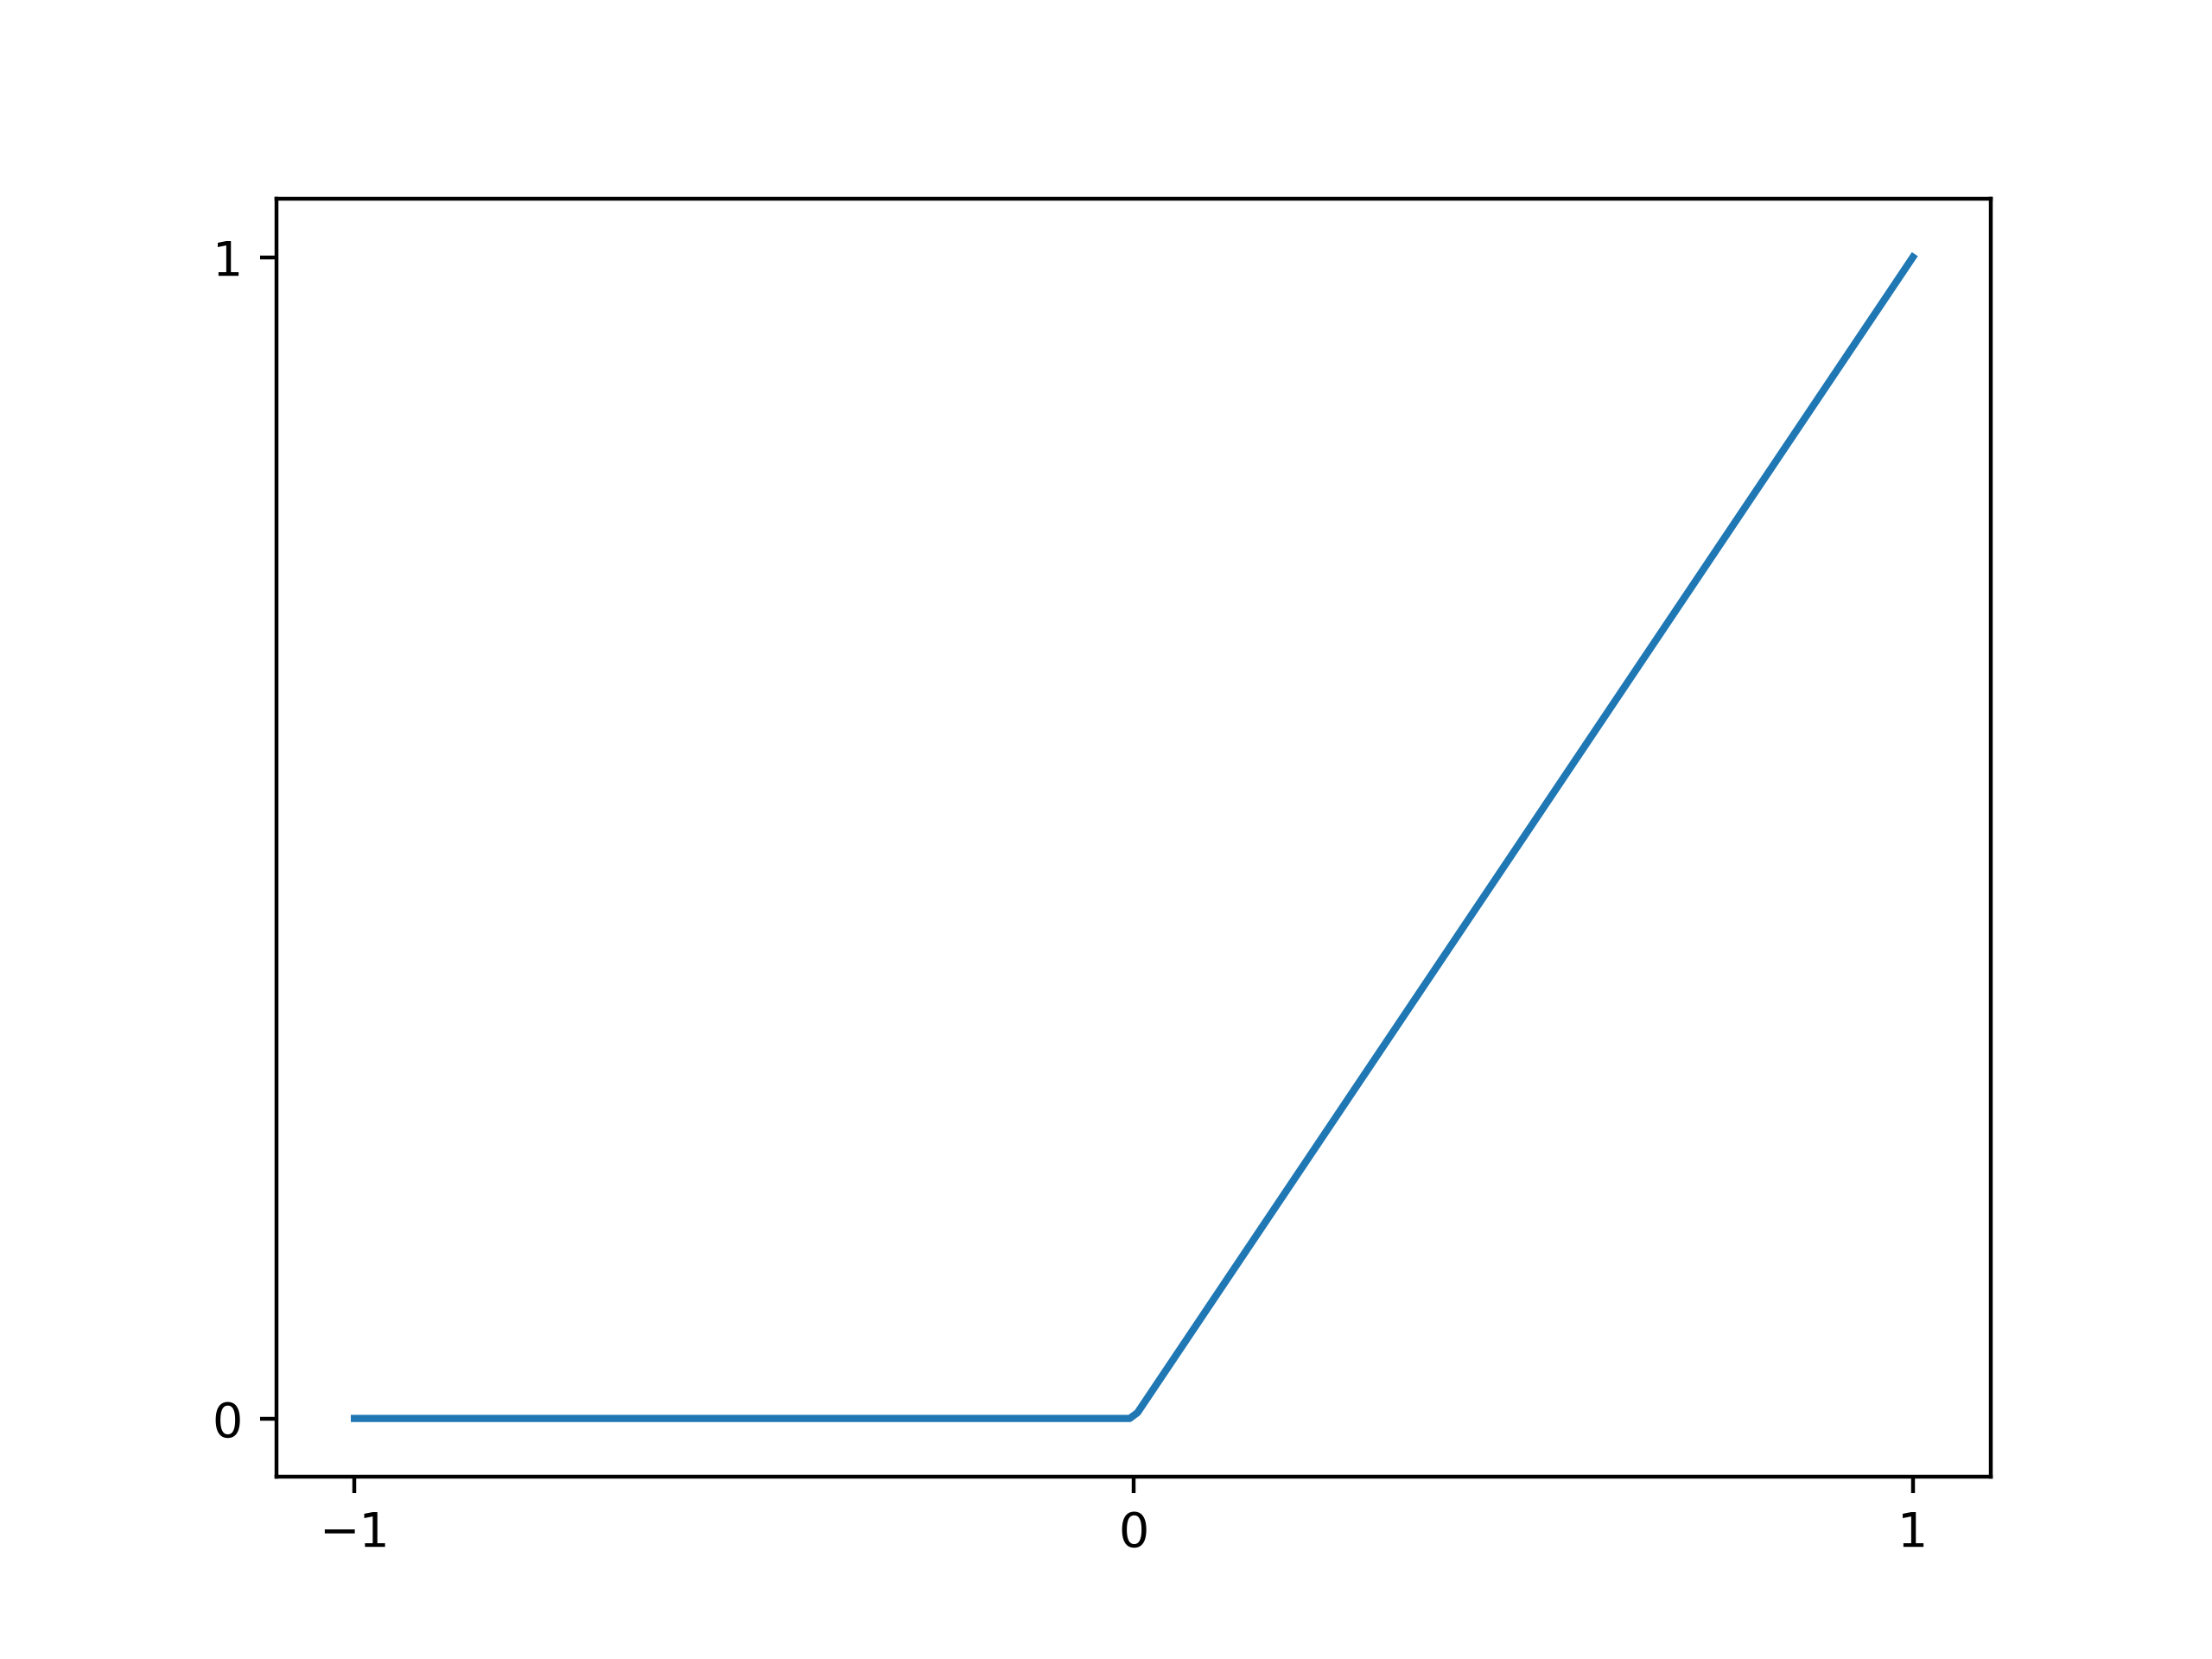
\includegraphics[scale=0.5]{relu.png} \\
	\end{tabular}
	\caption{放在table环境里则为表}
\end{table}
\begin{figure}[h]
	\center
	\begin{tabular}{cc}
		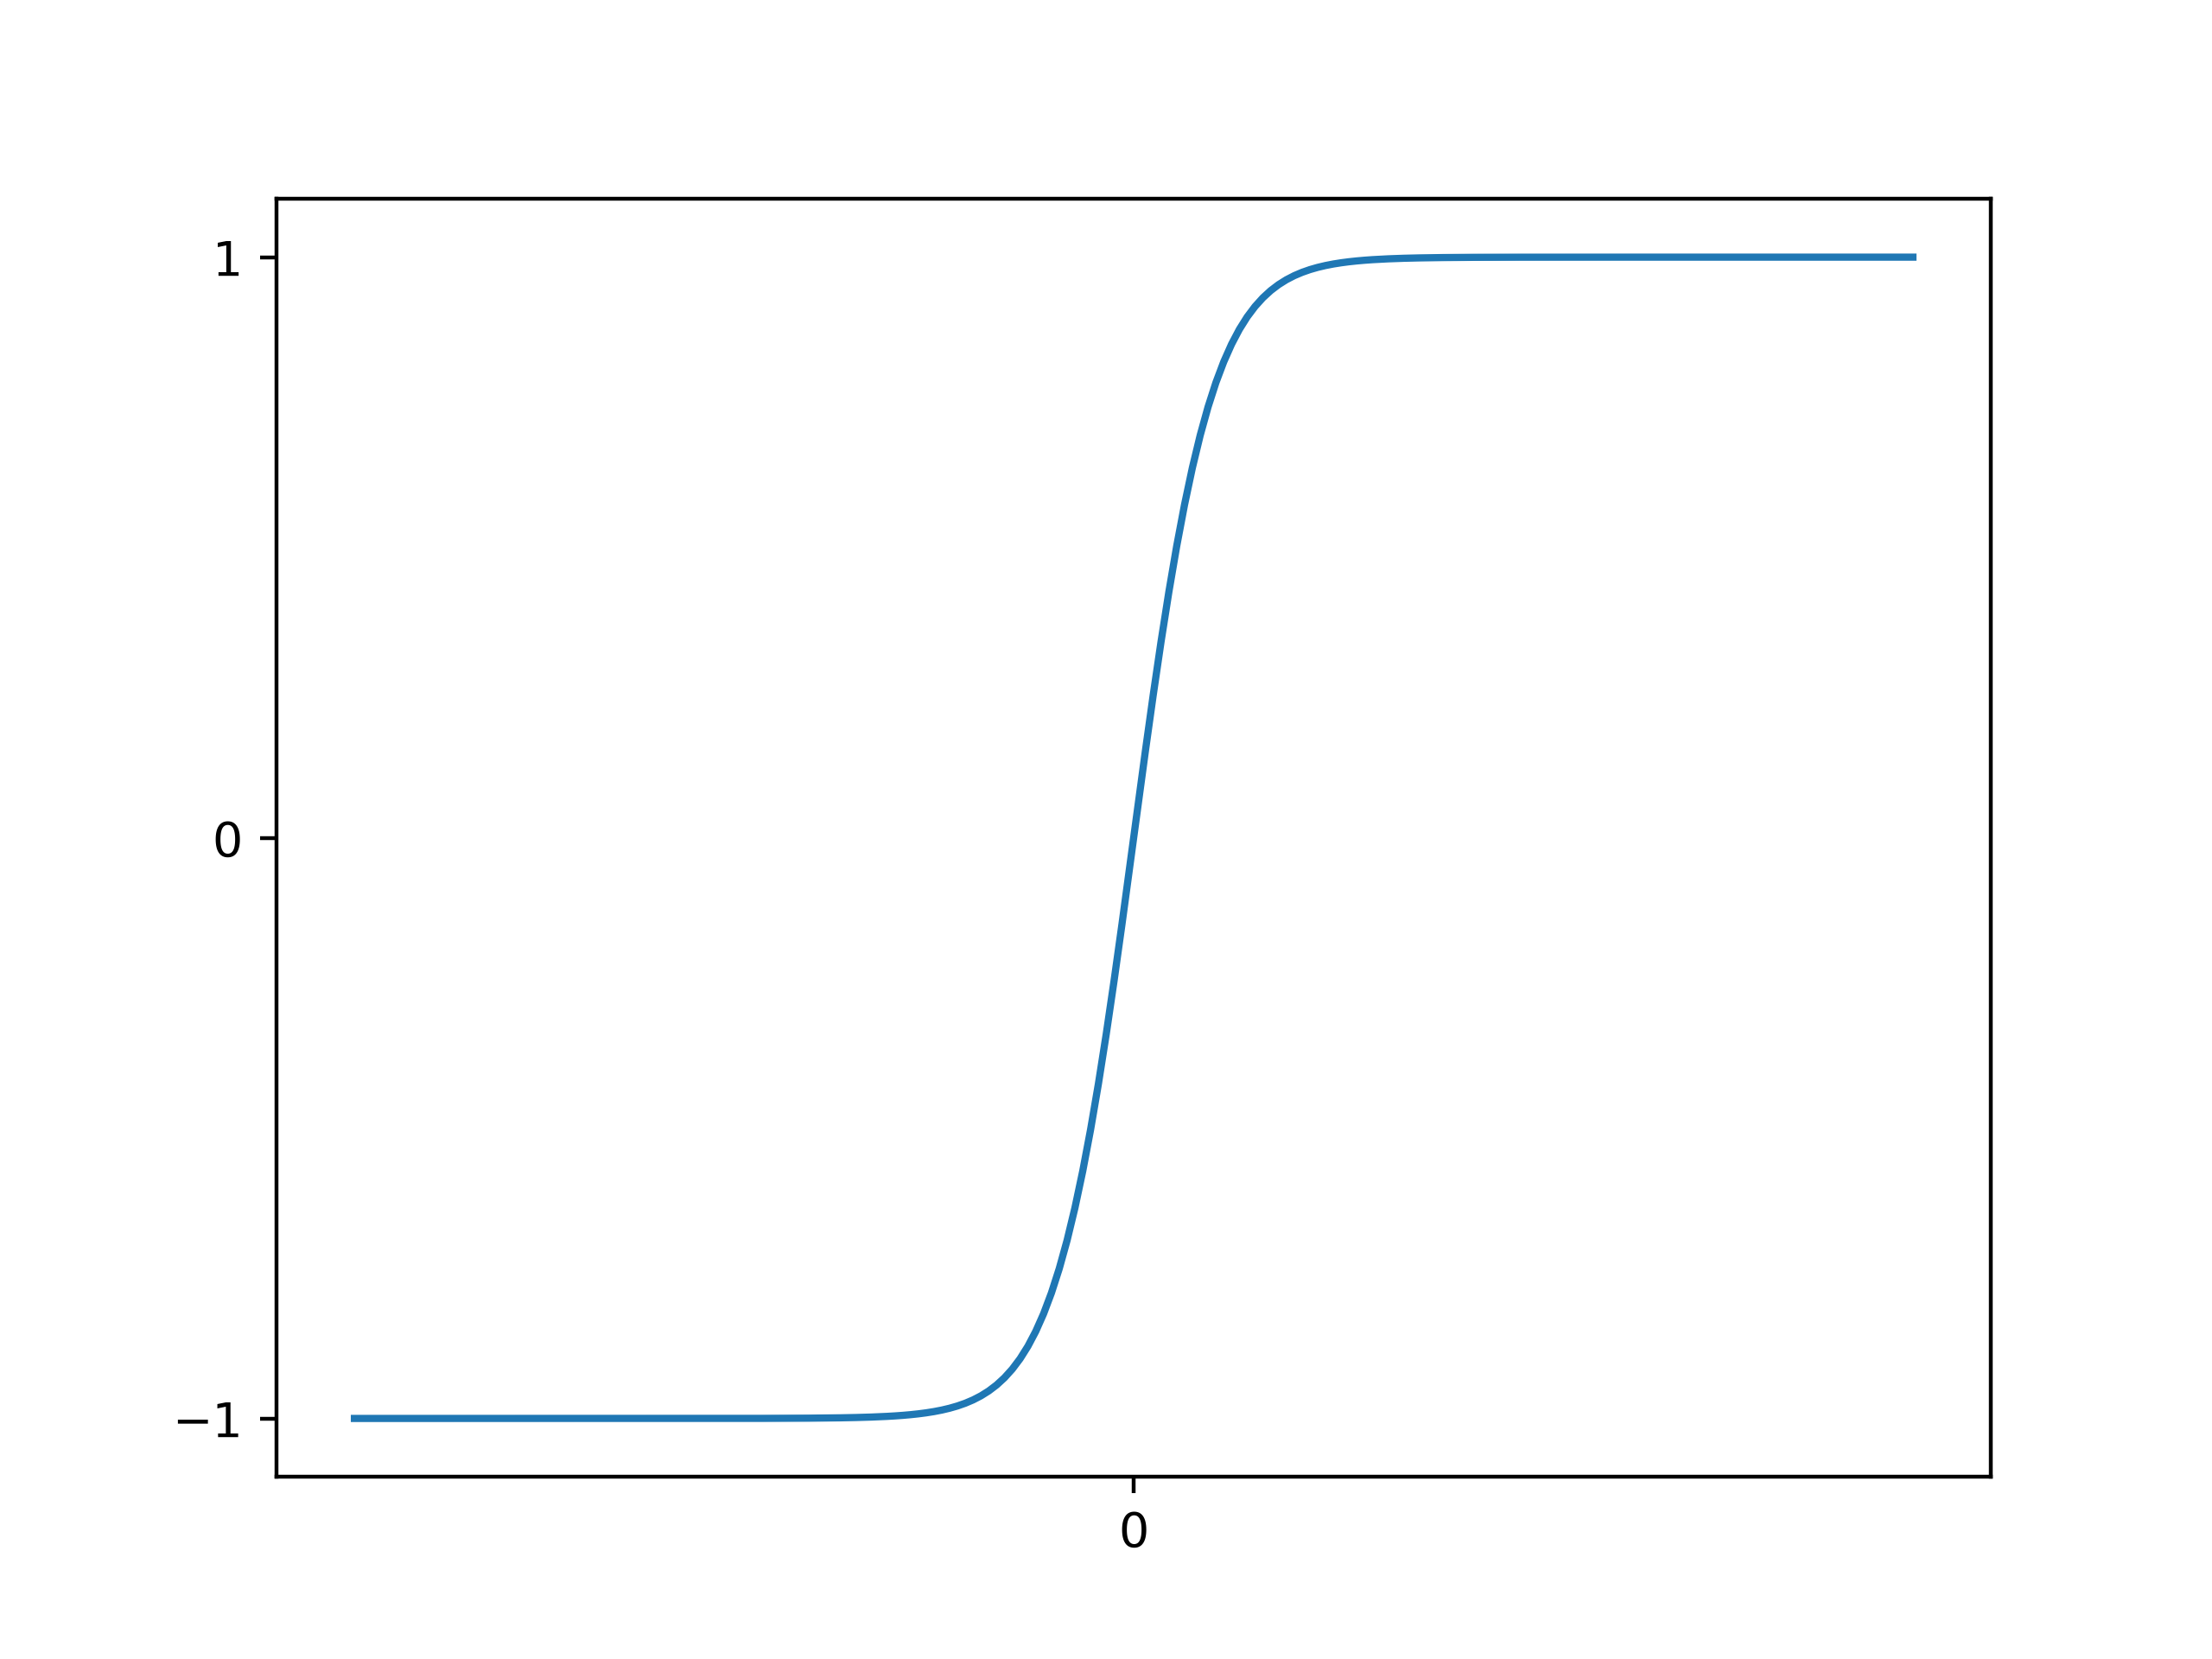
\includegraphics[scale=0.2]{tanh.png}
		 &
		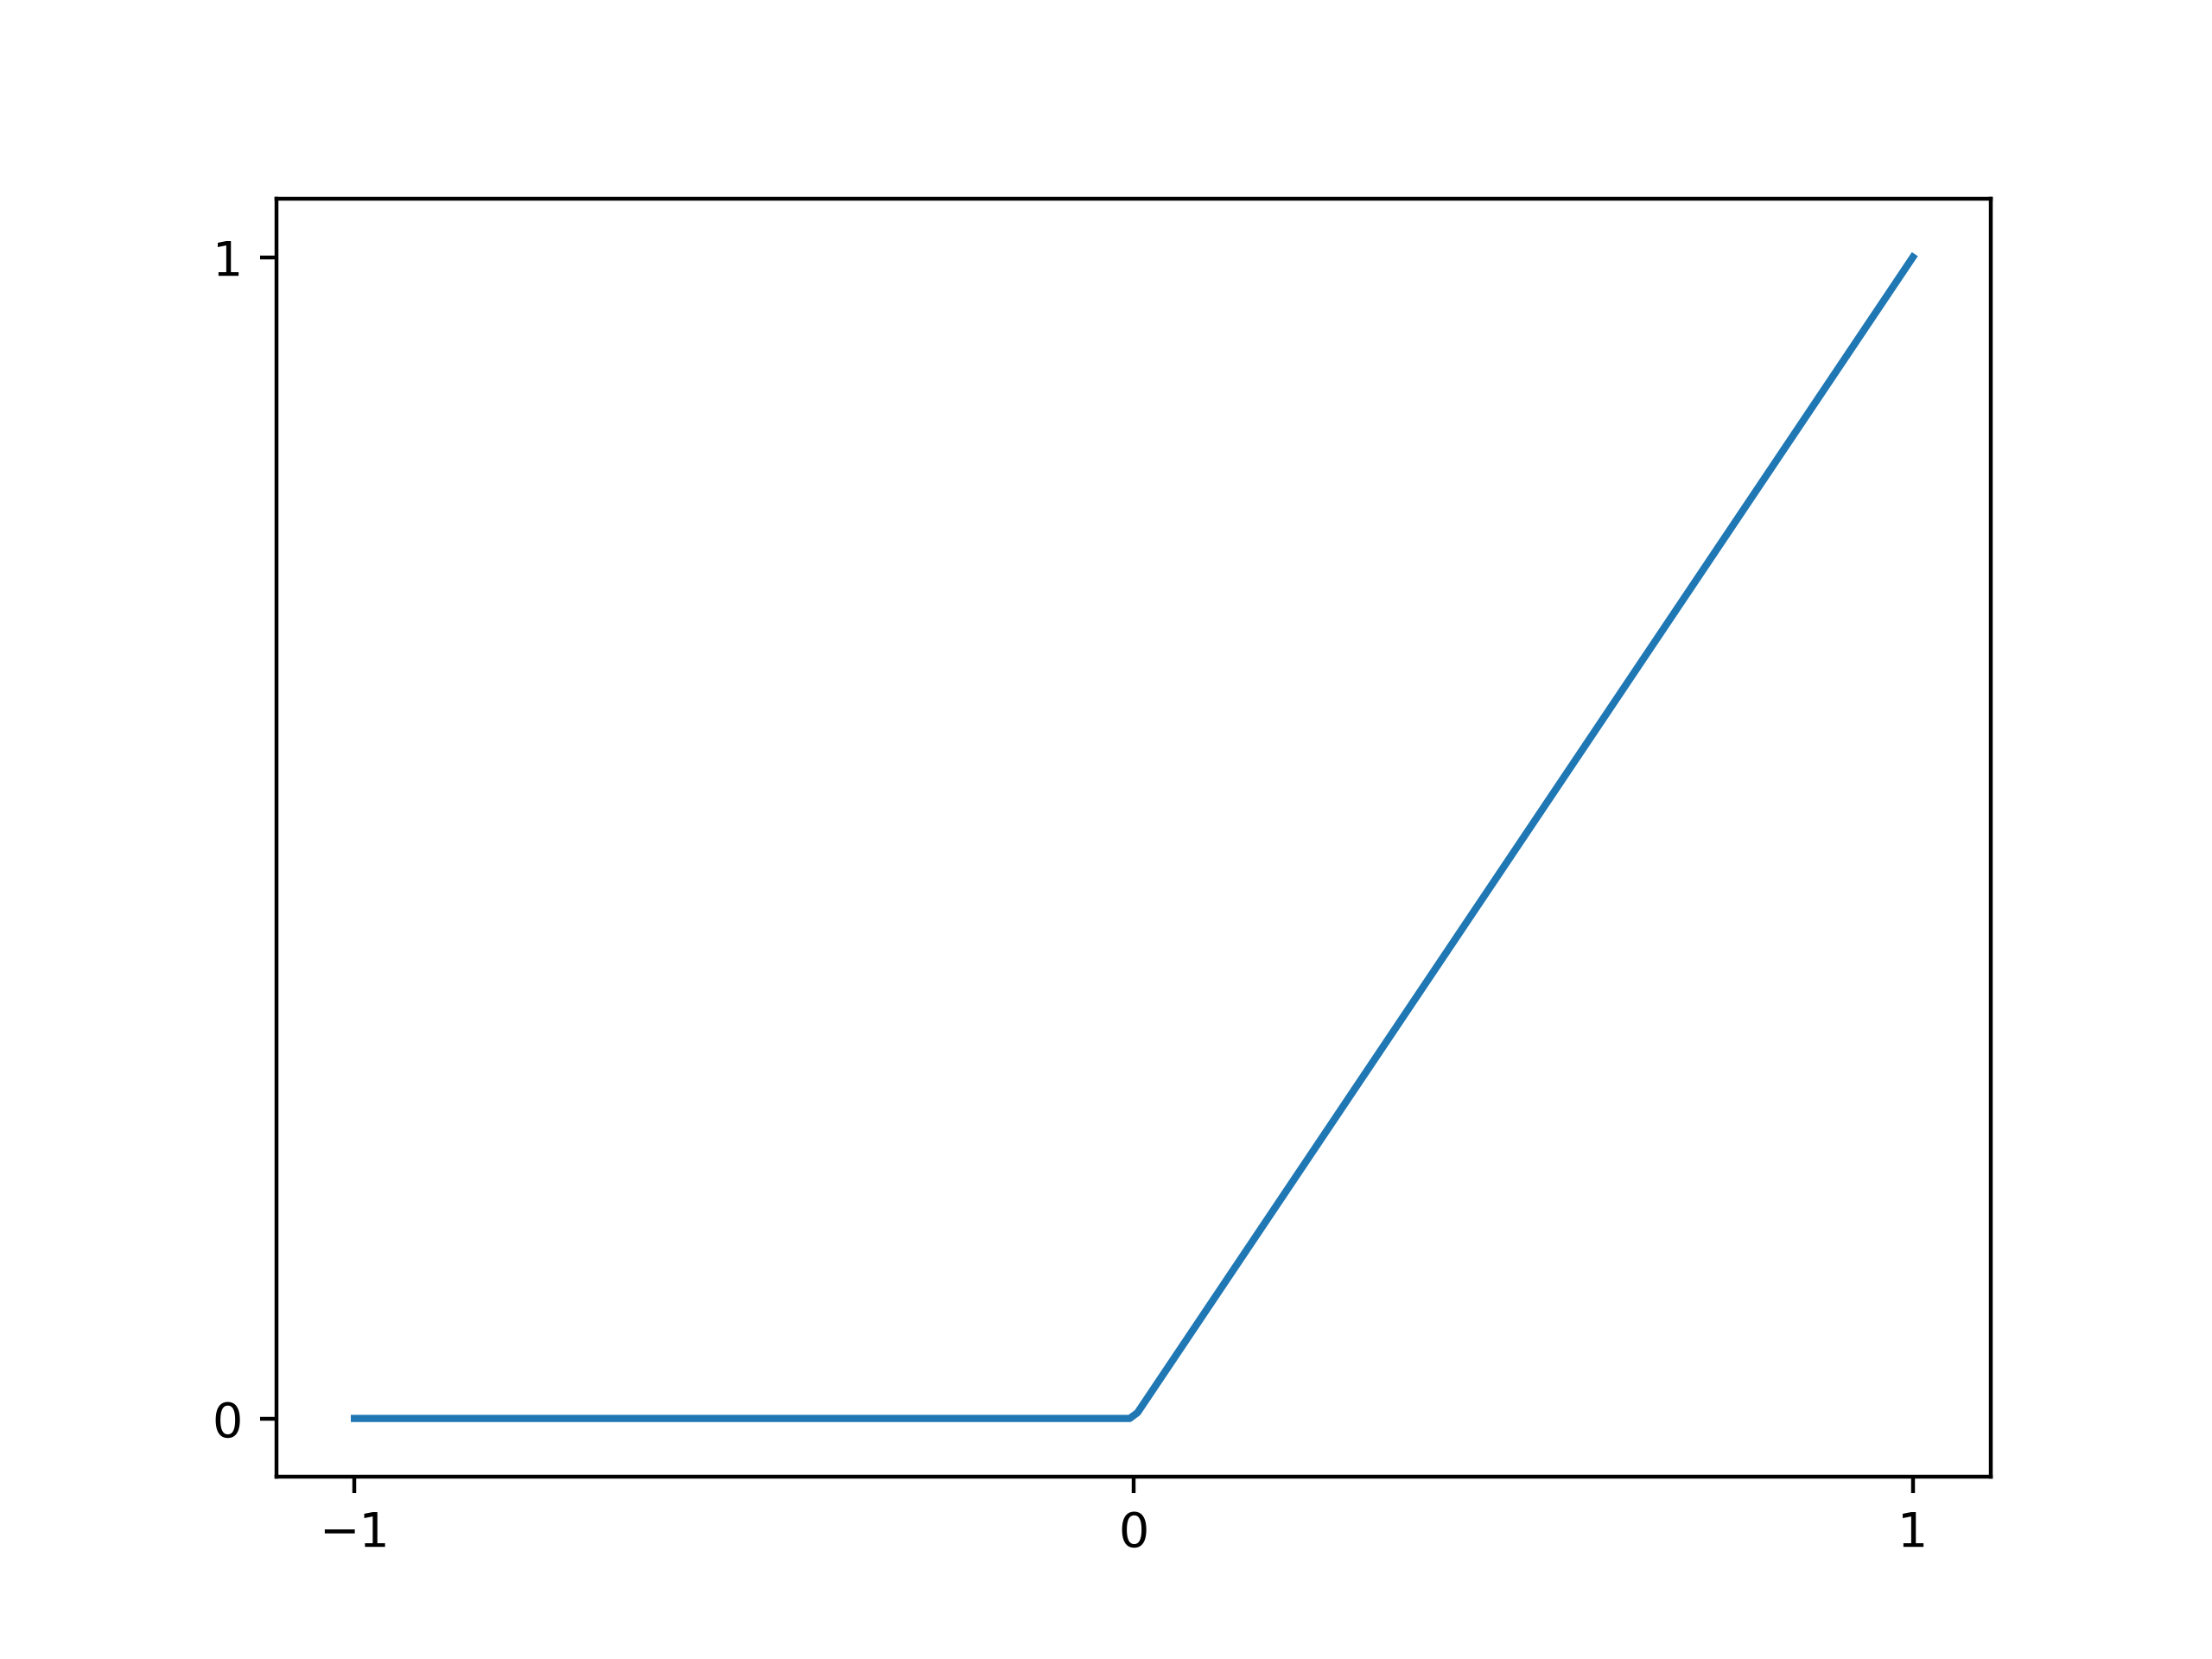
\includegraphics[scale=0.2]{relu.png} \\
		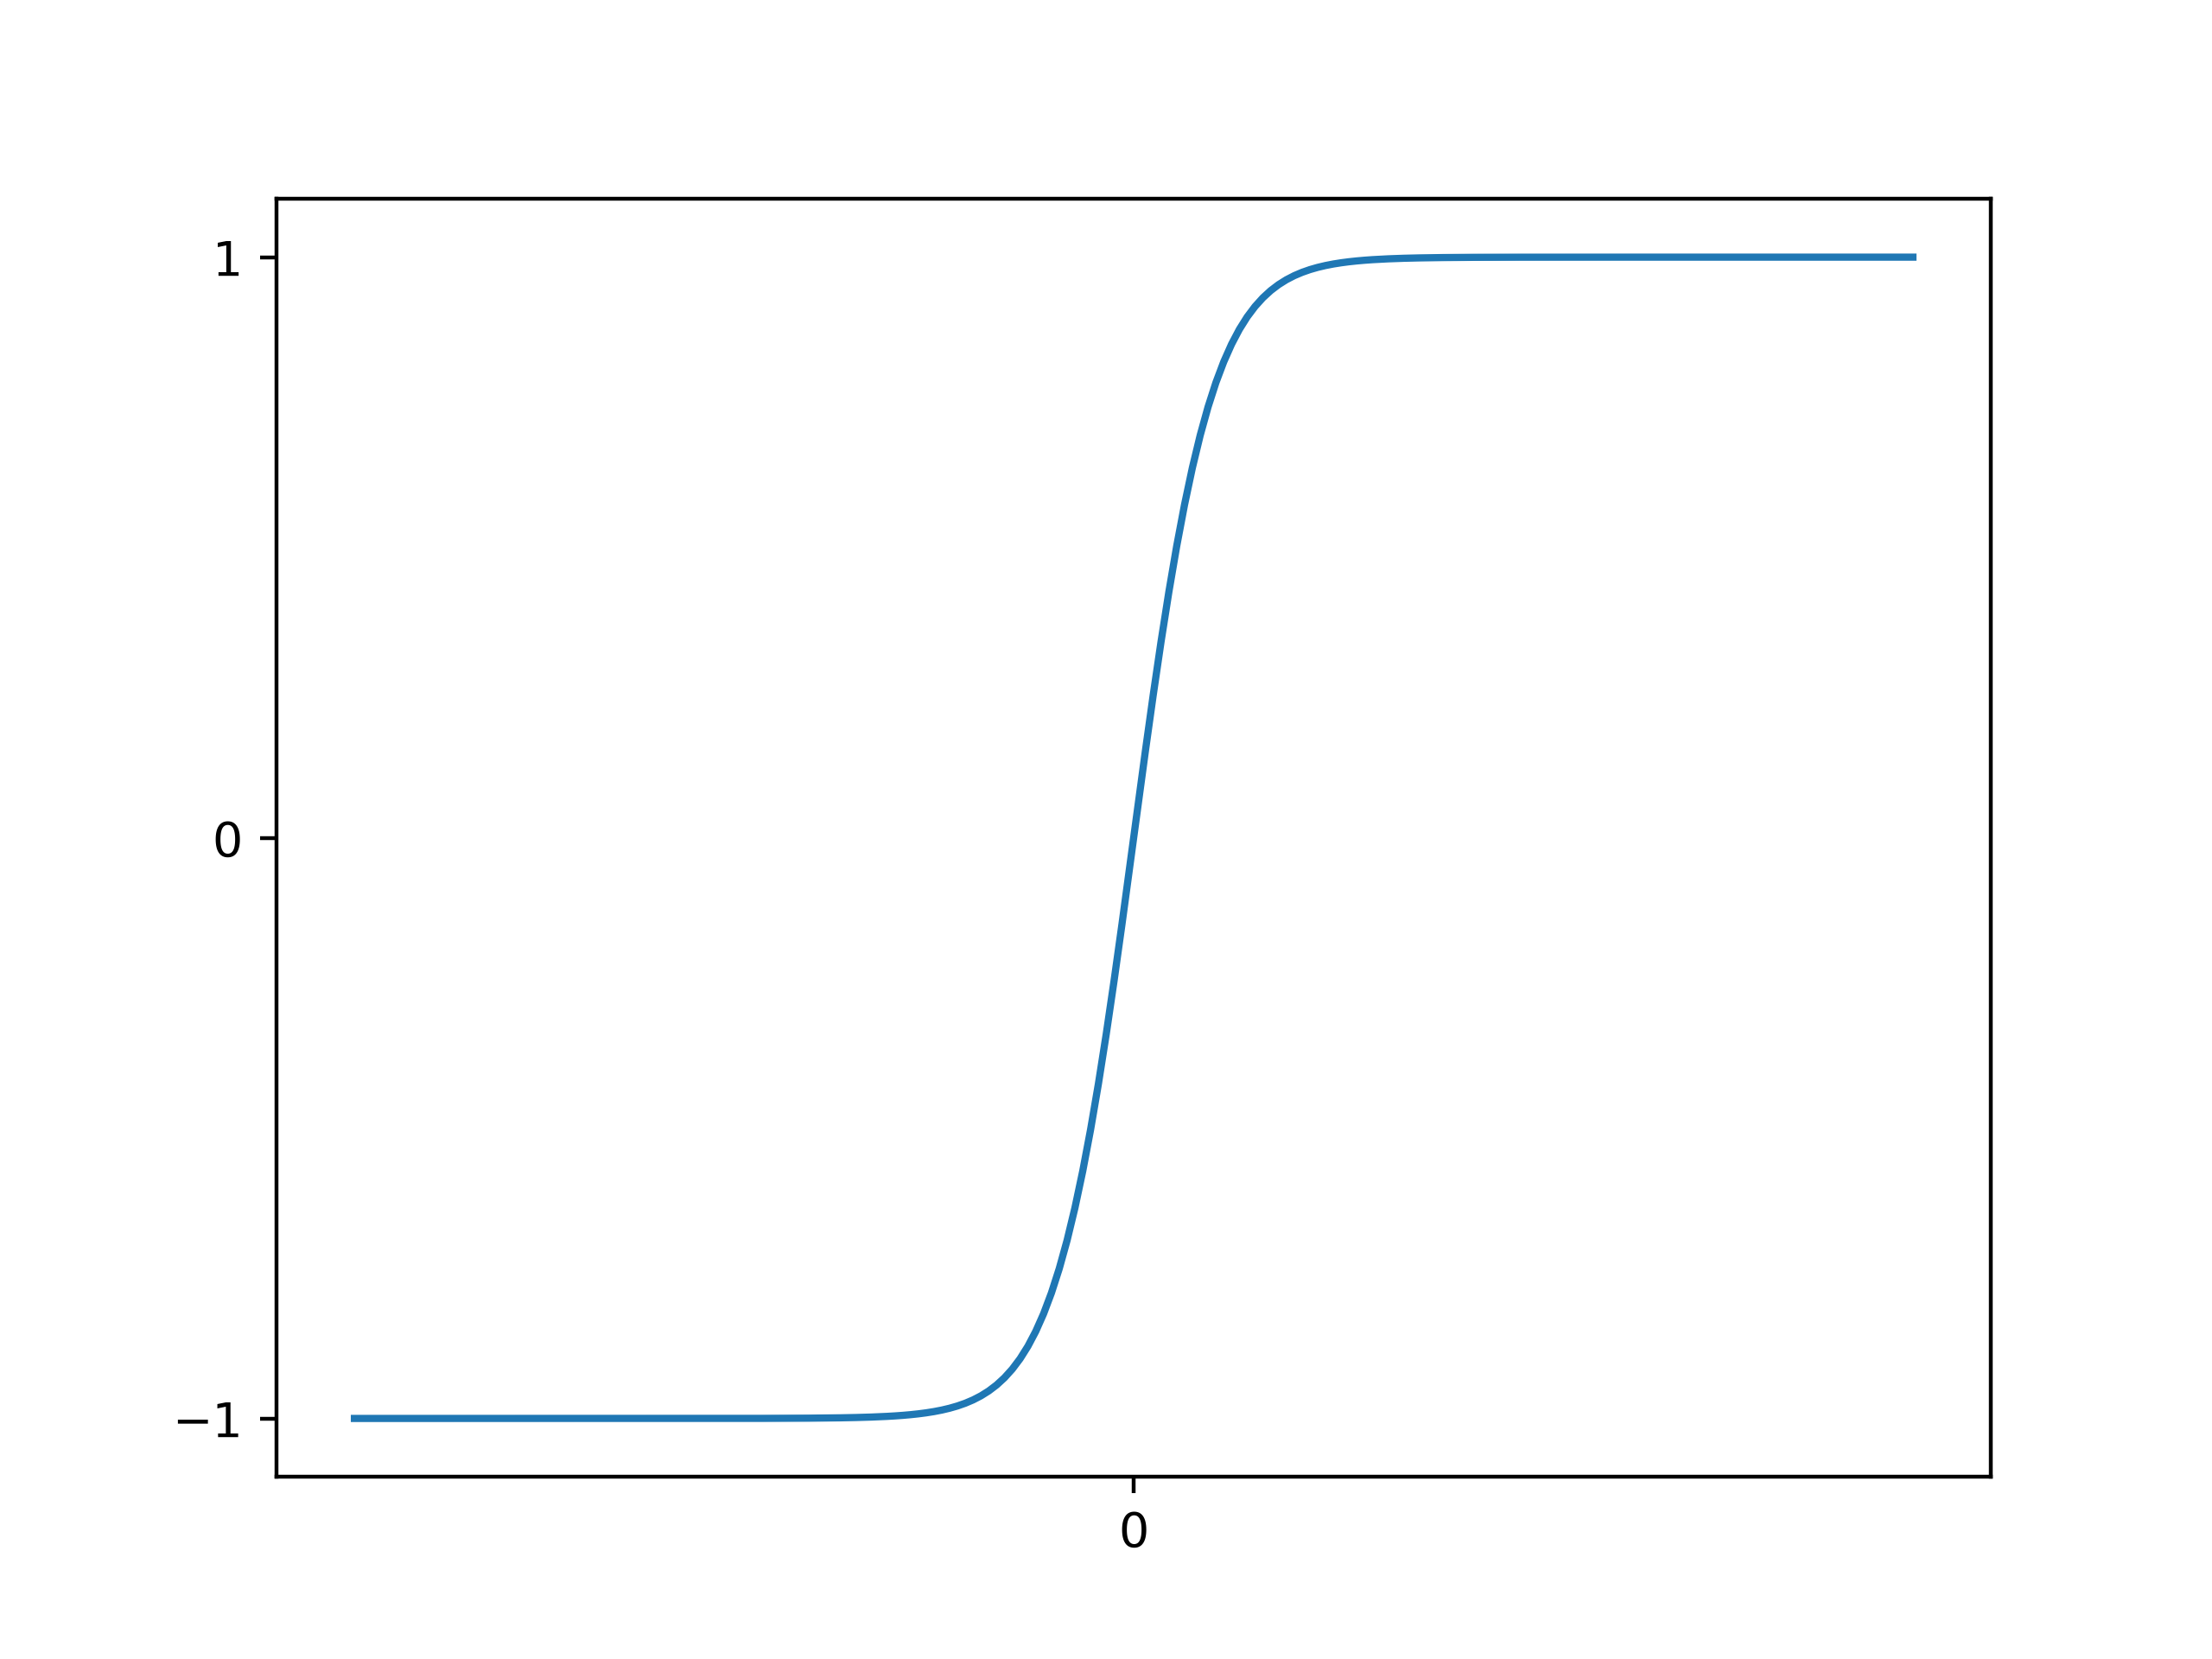
\includegraphics[scale=0.2]{tanh.png}
		 &
		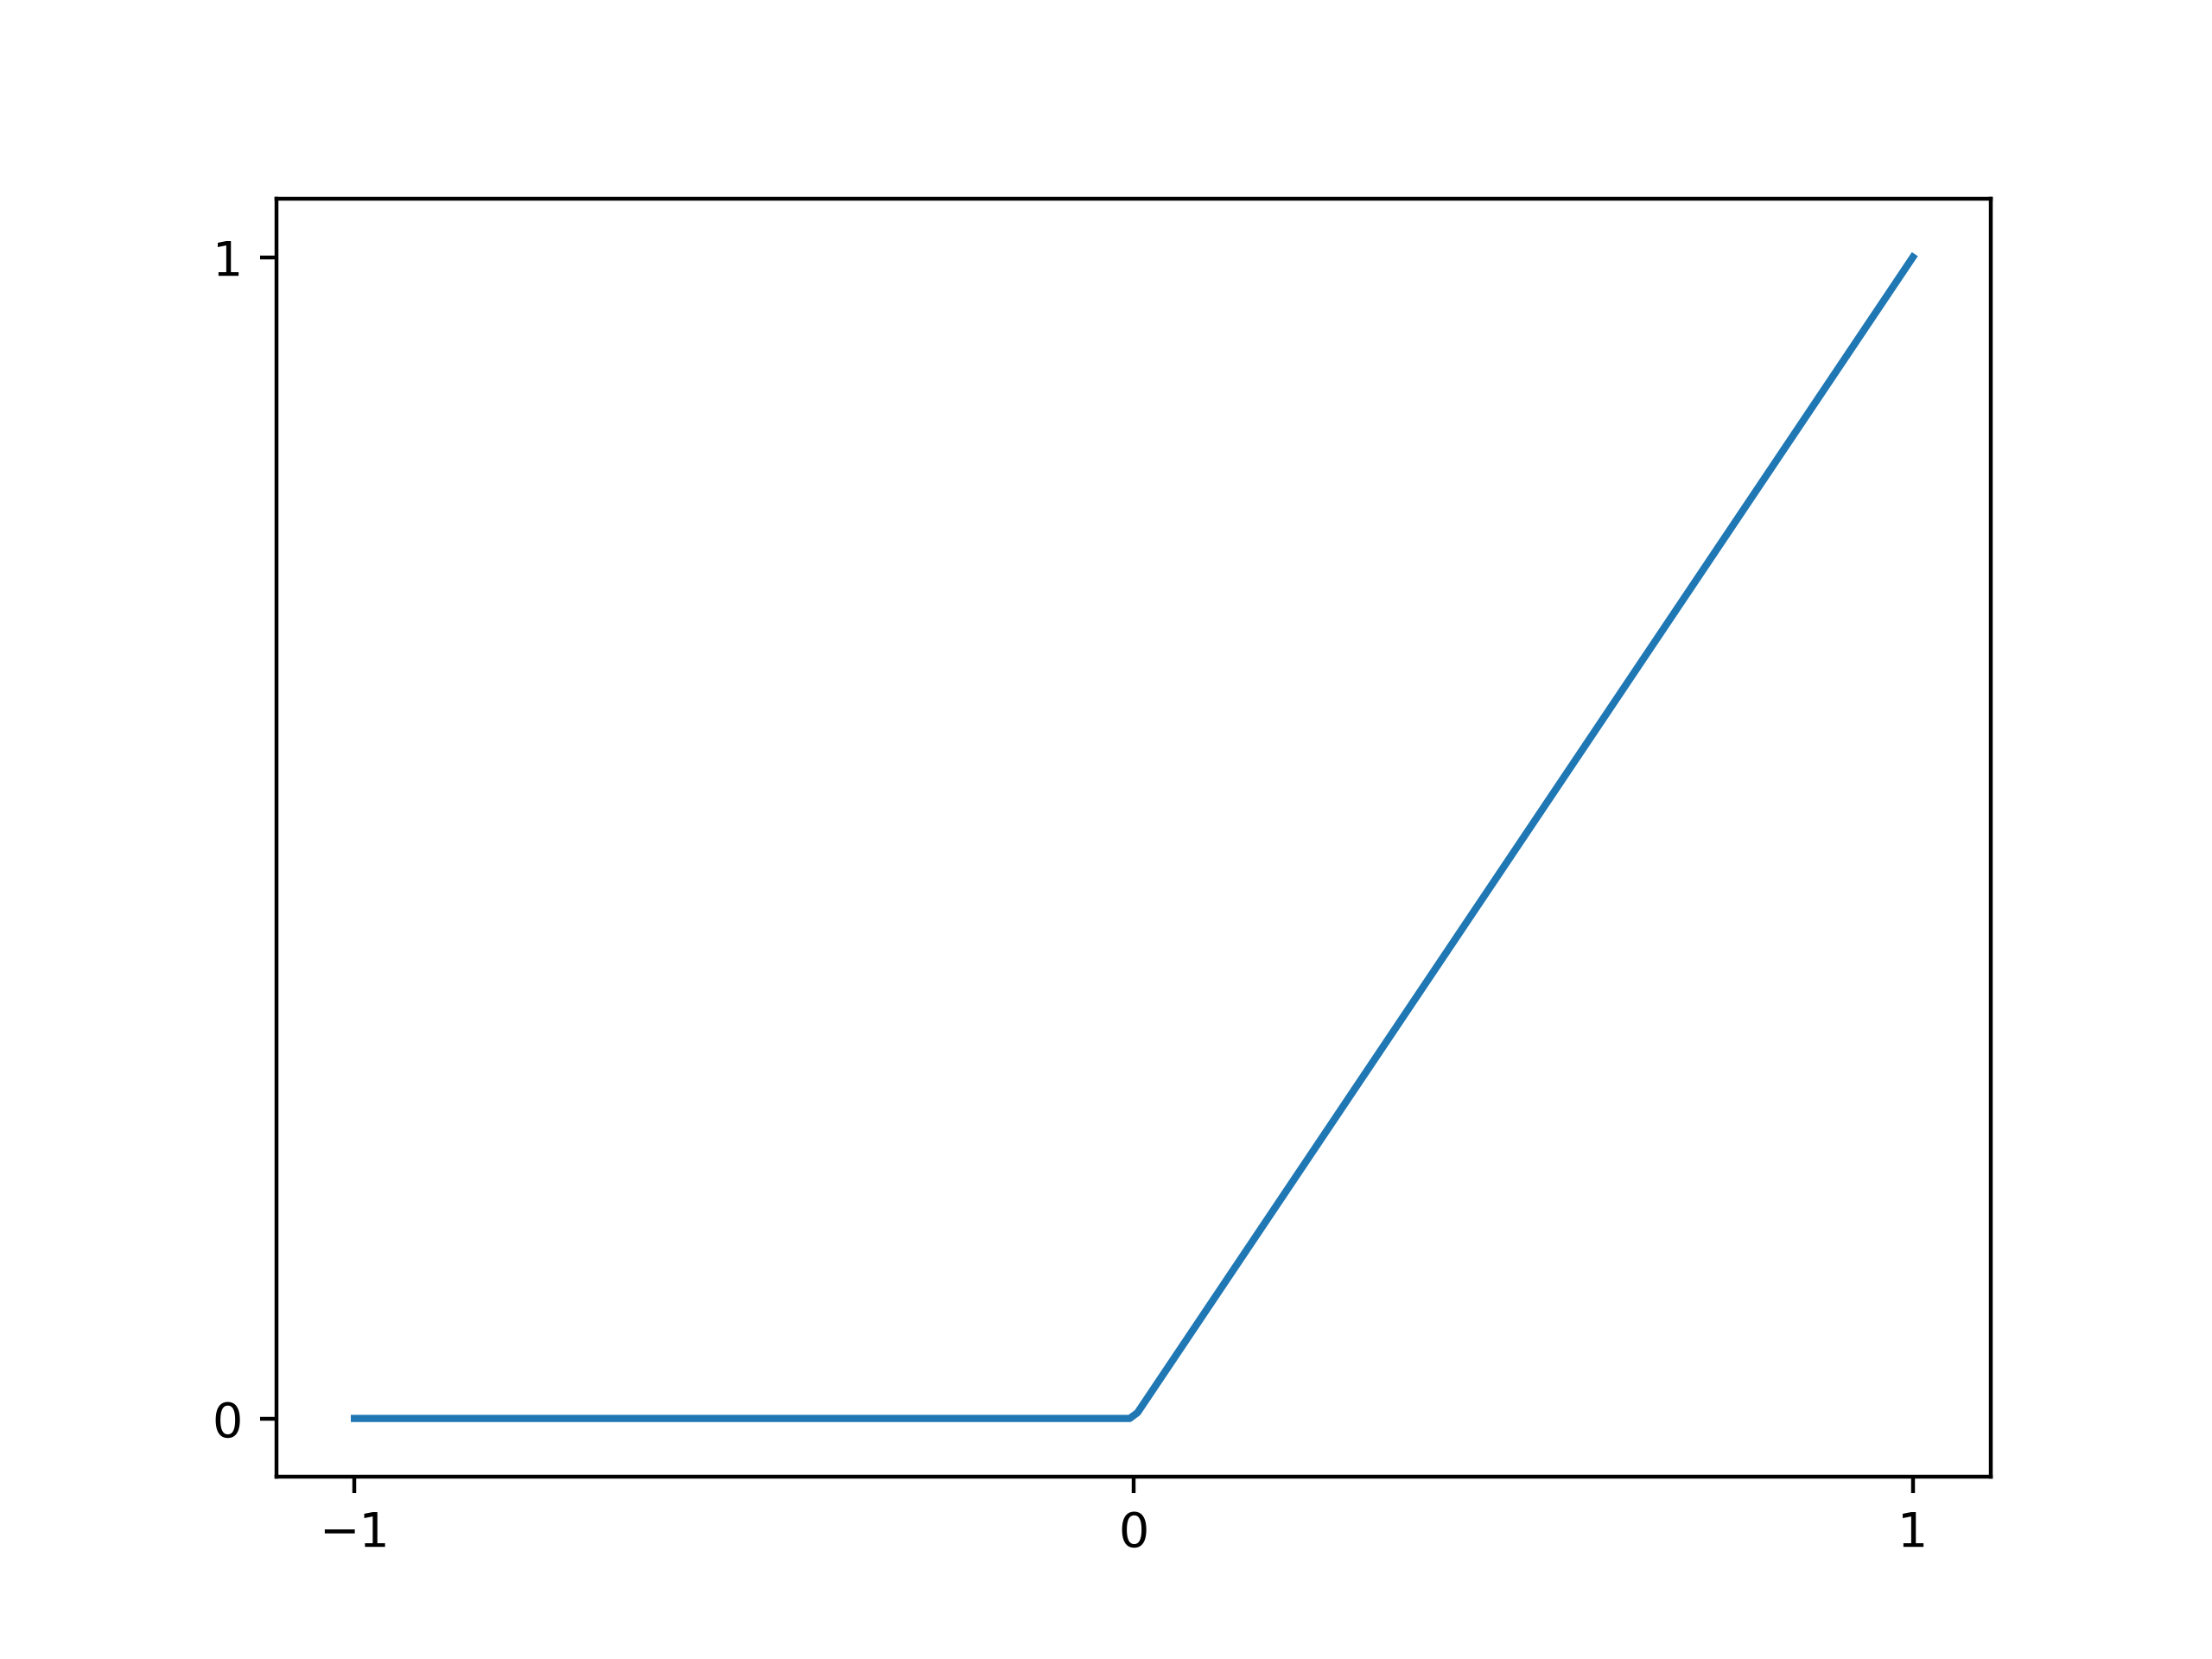
\includegraphics[scale=0.2]{relu.png} \\
	\end{tabular}
	\caption{放在figure环境里则为图}
\end{figure}

\begin{table}[htbp]
	\caption{跨列图}
	\center
	\begin{tabular}{ll}
		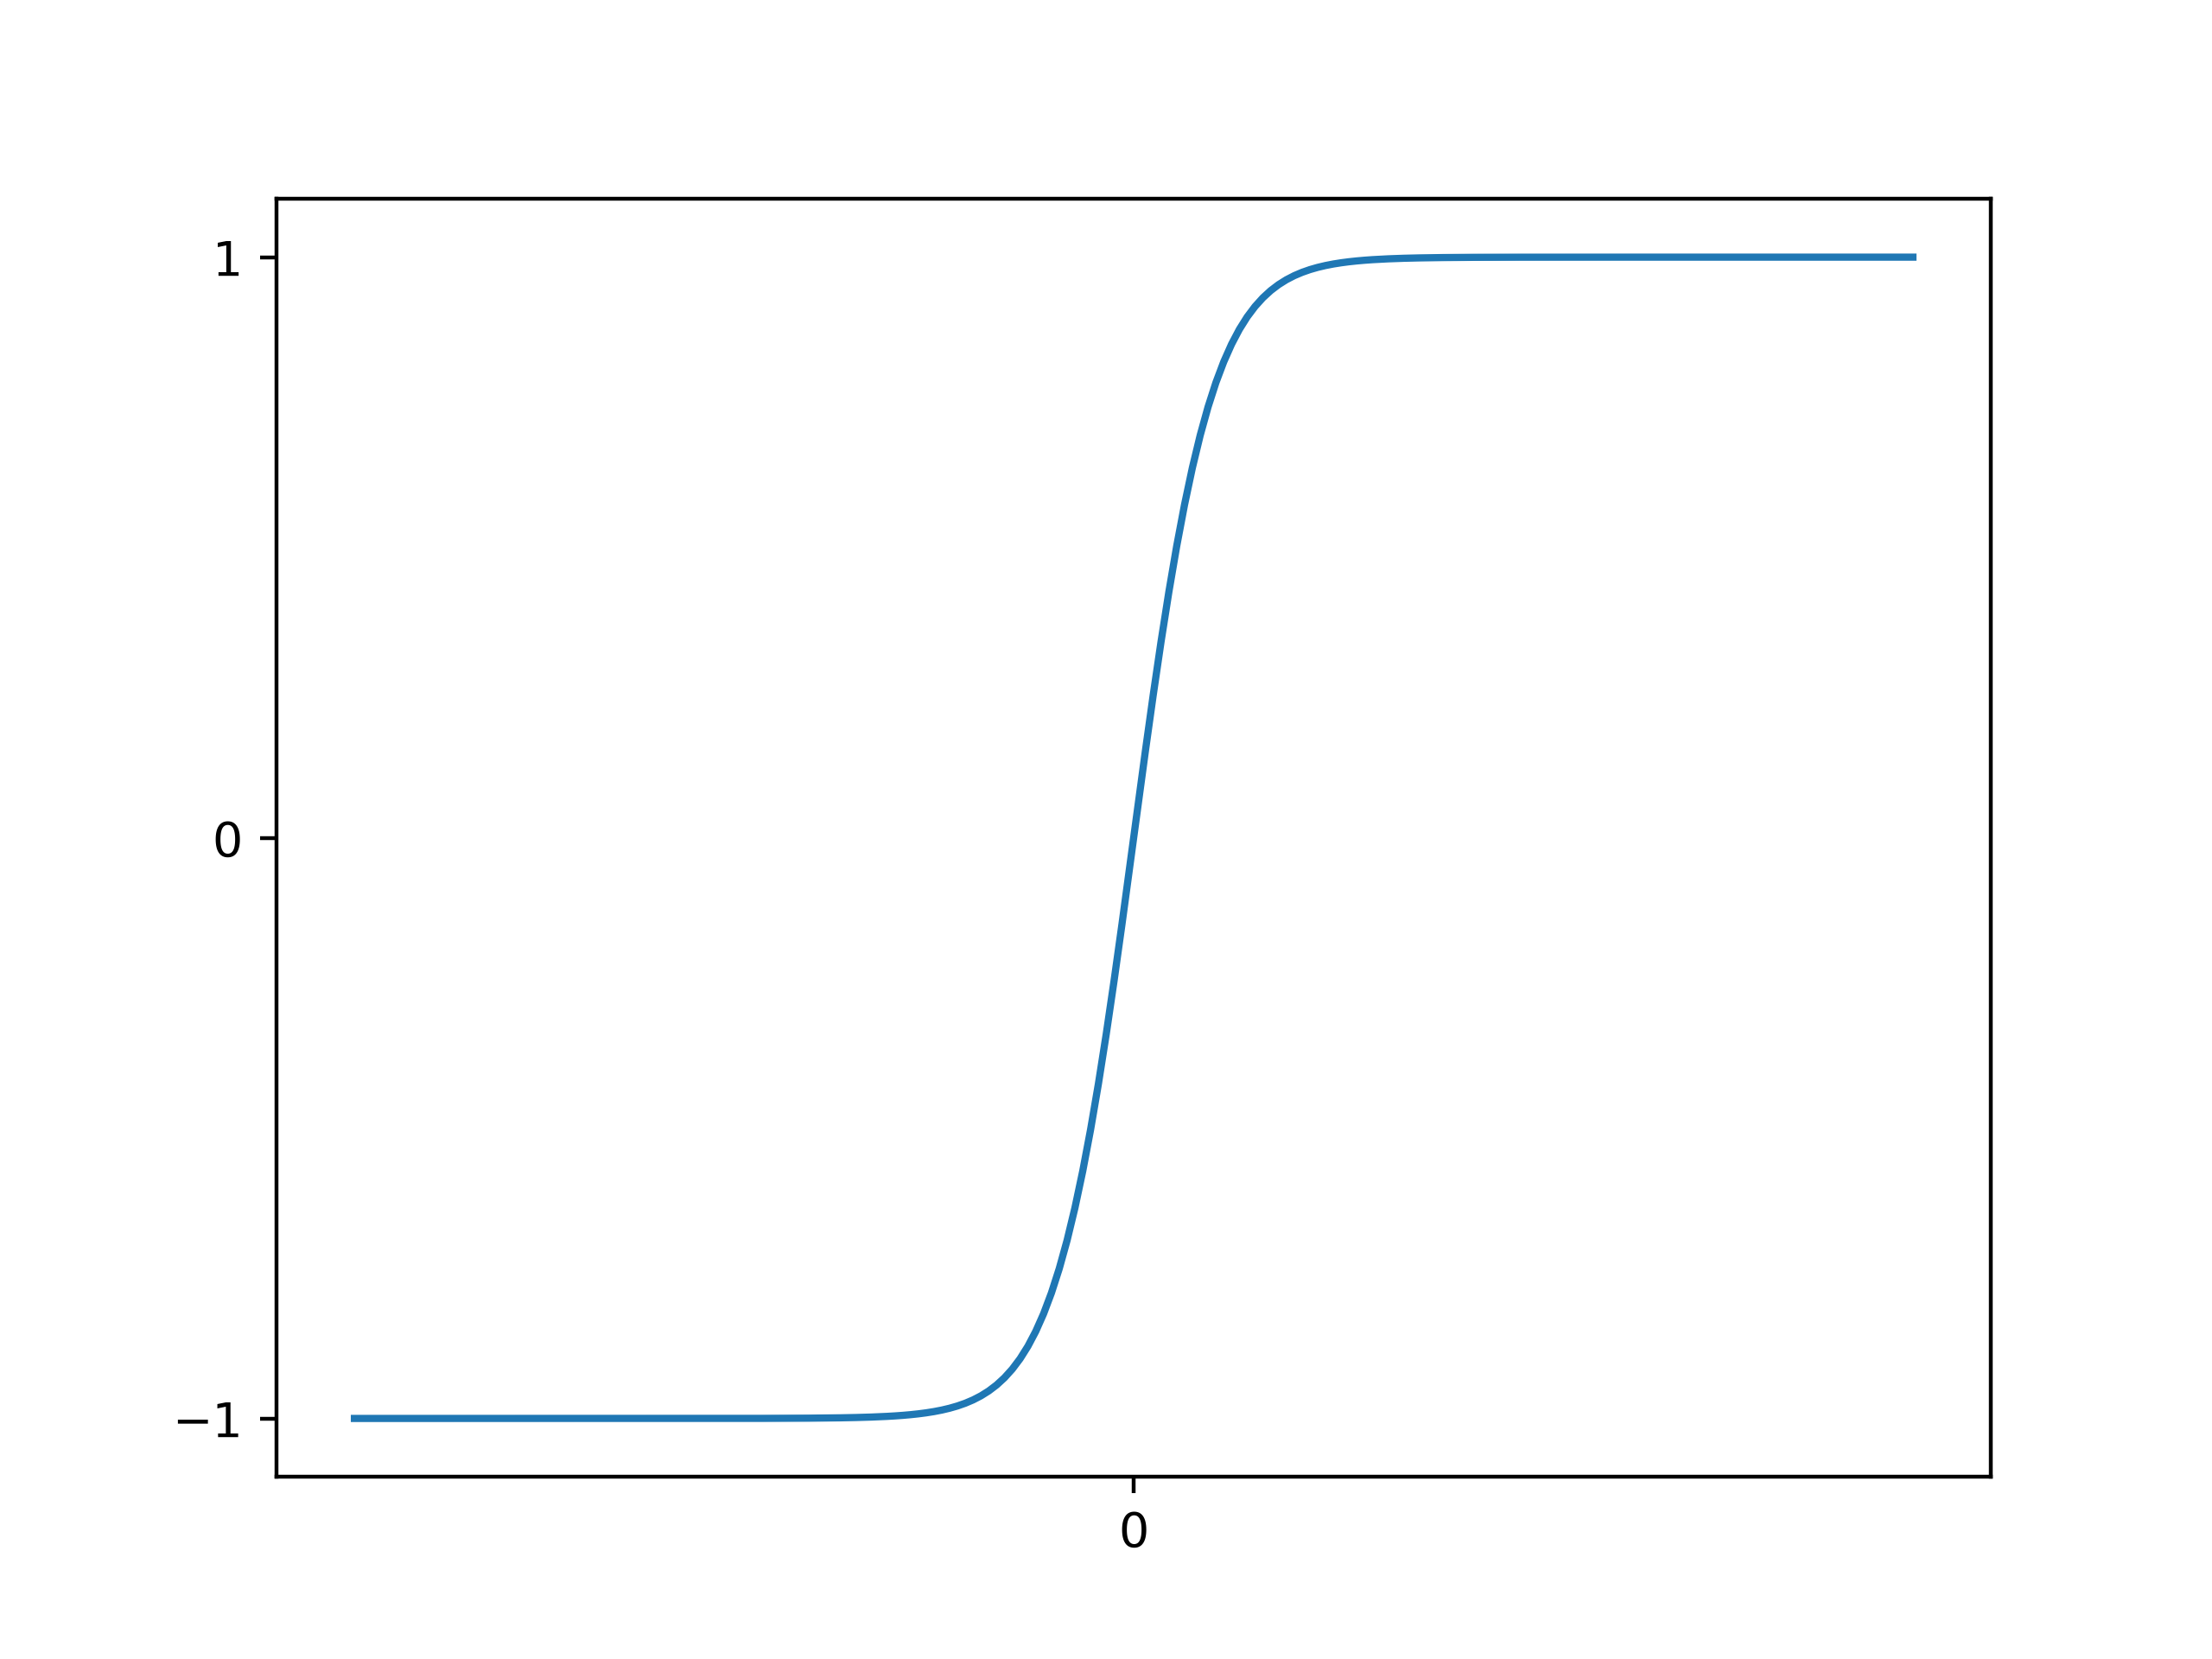
\includegraphics[scale=0.3]{tanh.png}
		 &
		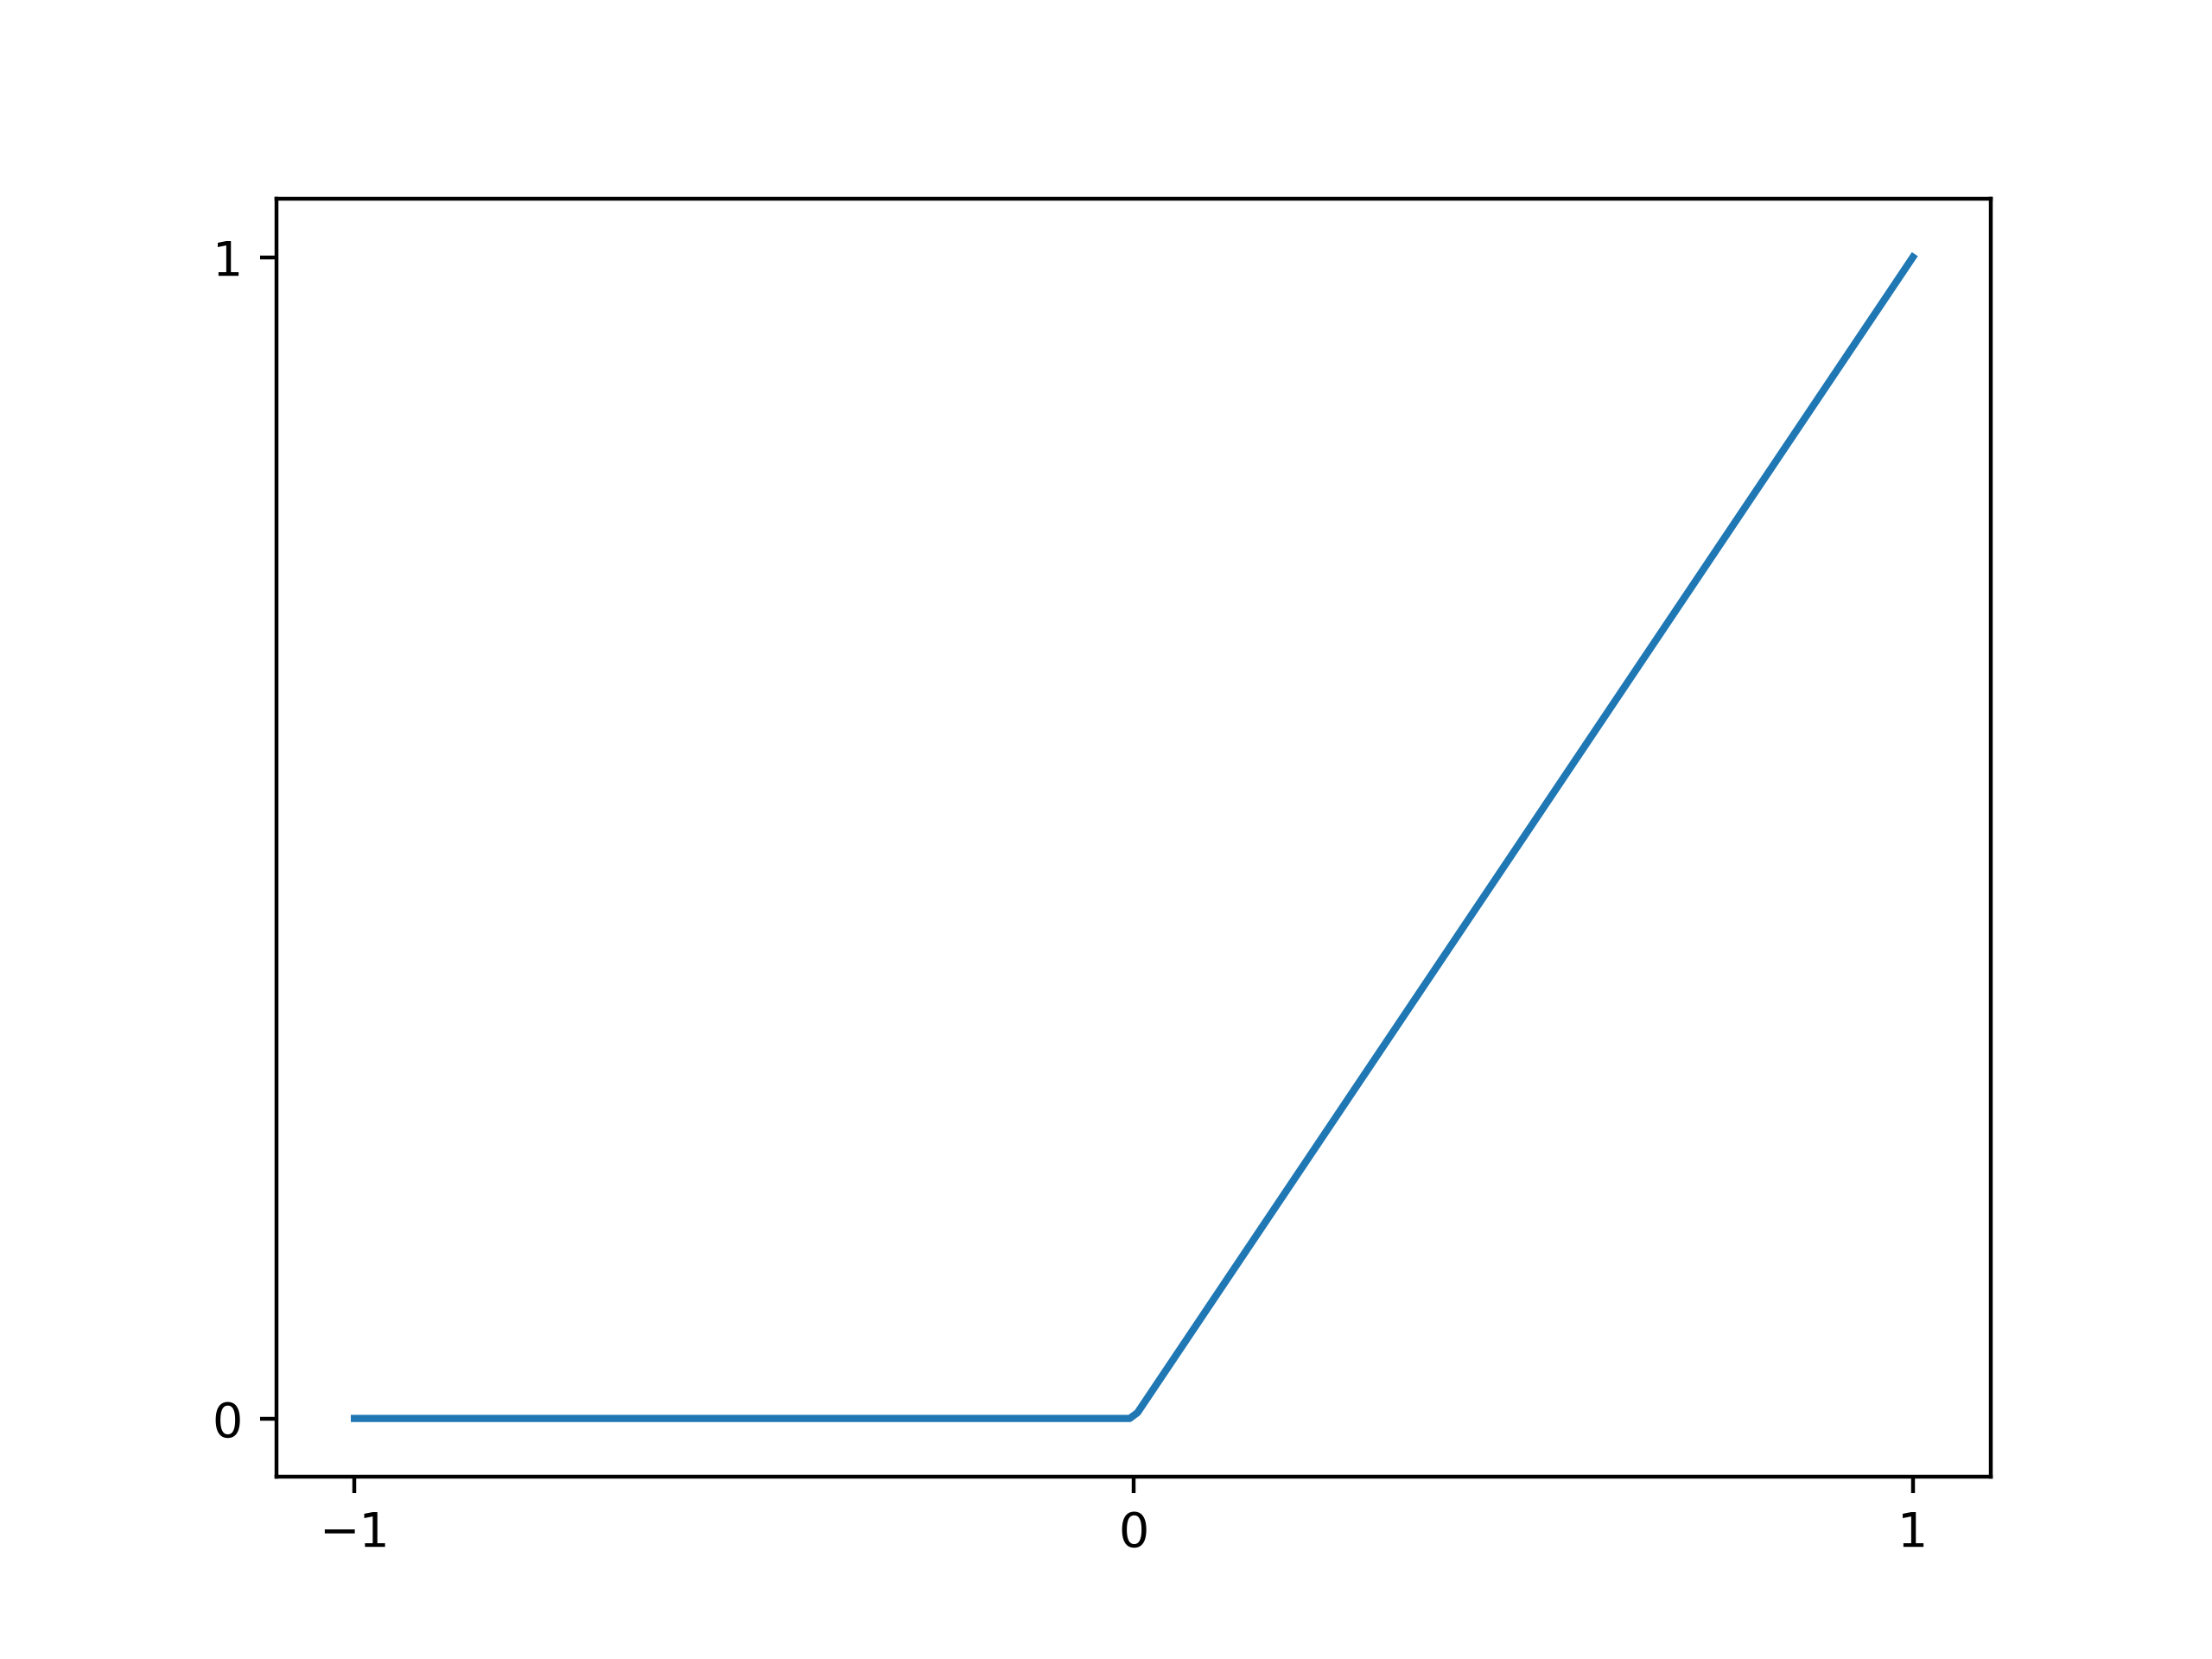
\includegraphics[scale=0.3]{relu.png} \\
		\multicolumn{2}{c}{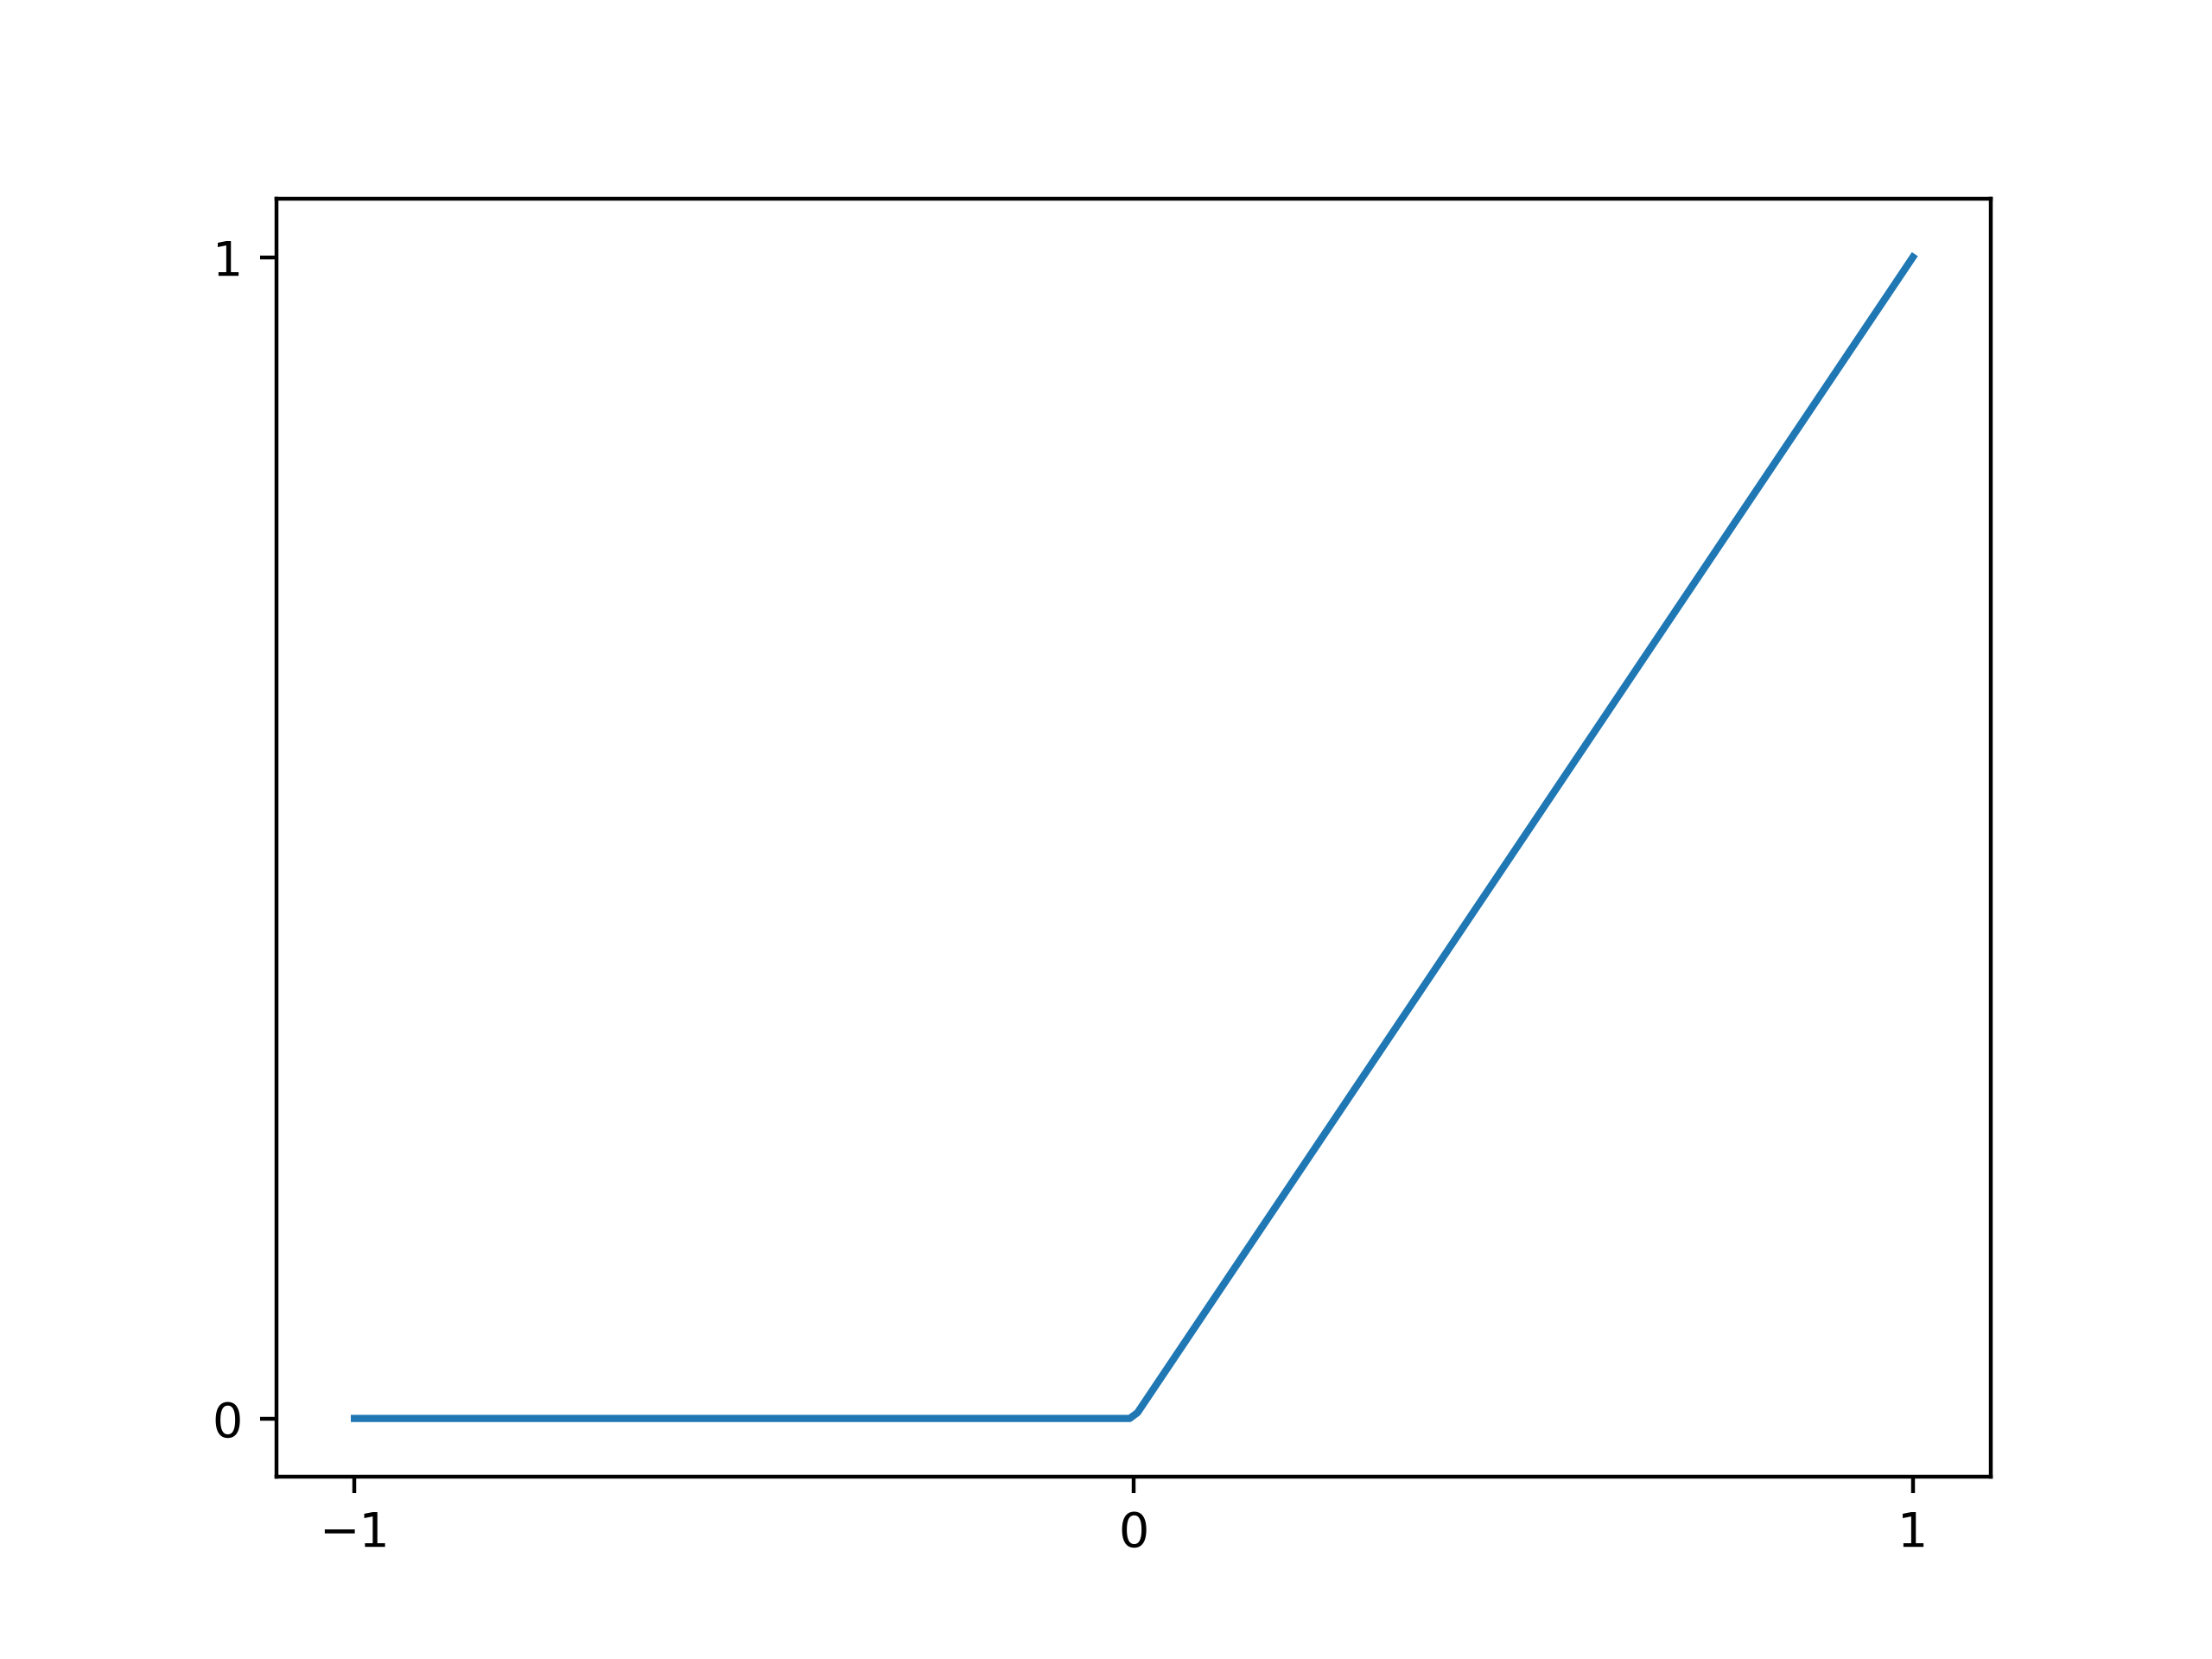
\includegraphics[scale=0.5]{relu.png}}
	\end{tabular}
\end{table}

\cleardoublepage
\bibliography{math} %加载同目录下文件名为math的.bib文件,生成参考文献
\end{document}


=================================================================
+																+
+																+
=================================================================

bibtex是专门用来处理latex参考文献的程序,使用是要经过四次编译
1. xelatex *.tex 生成辅助文件,确定数据库哪些文献将被列出(文献数据库本质为后缀为.bib的纯文本文件)
2. bibtex *.aux 从数据库选取文献,按指定格式生成参考文献列表
3. xelatex *.tex
4. xelatex *.tex 后两次生成正确的引用(否则引用为?,交叉引用也需要编译两次)

交叉引用:
\label{书签名} 书签命令,紧跟被引用对象之后,如章节,插图,表格标题之后,或文本,各种环境中
\ref{书签名} 序号引用命令,插在引用处,用于引用书签命令所在标题或环境的序号,或文本所在章节的序号
\eqref 引用公式
\pageref{书签名} 引用页码
为便于区别,书签名一般格式 fig:*

分文件编写:
正文使用\include{path}(path可以不带后缀.tex)
导言区使用\input(path)(\input相对于直接替换文本,如可以把自定义命令单独写一个文件,然后在导言区input)